\documentclass[12pt, letterpaper]{article}
\usepackage[utf8]{inputenc}
\usepackage{graphicx}
\usepackage{amsmath}
\usepackage{parskip}
\usepackage{tikz}
\usepackage{hyperref}

\newcommand{\externalLink}[2]{\emph{\underline{\href{#1}{#2}}}}


\title{Notes on Calculus III}
\author{Aaron Pierce}
\date{} % to remove date from \maketitle
\begin{document}

\maketitle

\tableofcontents

\newpage

\section{Early Chapters}

The beginning chapters aren't as noteworthy as the later ones, but they are still valuable. The following is a collection of the most important or interesting parts

\subsection{Dot Products}
Dot products are a form of vector multiplication. 

\textbf{Definition:} The dot product of two vectors ($\vec{A} \cdot \vec{B}$) is a real number given by the length of the projection of one vector onto another times the length of the vector being projected on.

That's a mouthful, and I like pictures.

\begin{figure}[h]
    \centering 
    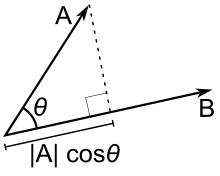
\includegraphics[width=0.30\textwidth]{dotproduct}
    \caption{A dot product in progress, as A is being projected onto B}
\end{figure}

Numerically, this projection is $|\vec{A}| cos(\theta) |\vec{B}|$, which corresponds to the length of the component of A that lies on B, times the length of B.

This definition derives some very useful other expressions, such as 

\begin{equation}
    \cos(\theta) = \frac{\vec{A} \cdot \vec{B}}{|\vec{A}||\vec{B}|}
\end{equation}
\begin{equation}
    comp_{\vec{B}} \vec{A} = \frac{\vec{A} \cdot \vec{B}}{|\vec{B}|} = \vec{A}\cos(\theta)
\end{equation}

\label{equOfDotProductDefinitions}
Another way to define the dot product is the sum of the products of the components of the vectors. Another mouthful. The math is a easier to understand
\begin{gather*}
    \text{Let} \vec{A} = (A_1, A_2, ..., A_n)\\
    \text{Let} \vec{B} = (B_1, B_2, ..., B_n)\\
    \vec{A} \cdot \vec{B} = A_1 B_1 + A_2 B_2 + ... + A_n B_n
\end{gather*}
Let's call this the algebraic definition, as opposed to the projection or geometric definition from earlier.\\
This was surprising to me. How is this equivalent to the projection definition from earlier?
What helped me was realizing that this definition is equivalent to applying the geometric definition over the components of B.

\begin{gather*}
    \text{Let} \vec{A} = (A_1, A_2, A_3)\\
    \text{Let} \vec{B} = (B_1, B_2, B_3)\\
    \vec{B} = (B_1, 0, 0) + (0, B_2, 0) + (0, 0, B_3)\\
    \vec{A} \cdot \vec{B} =  \vec{A} \cdot (B_1, 0, 0) + \vec{A} \cdot (0, B_2, 0) + \vec{A} \cdot (0, 0, B_3)\\
    = A_1 B_1 + A_2 B_2 + A_3 B_3
\end{gather*}

This amounts to projecting A onto each component of B, which is just the corresponding component of A (projecting a vector onto a vertical vector is the same as taking the vertical component of the first vector and so on), 
multiplying their lengths, and adding all of those multiplications up, which gives us exactly the algebraic definition of the dot product


\subsection{Cross Products}
Cross products are, in my head, the counterpoint to a dot product. Whereas you can think of the dot product as what two vectors have in common (the component of one on another), the cross product gives the opposite, what the vectors do not have in common

Yet again we have two definitions, a geometric definition (again preferred by me), and an algebraic one

\textbf{Geometric Definition:} The cross product of two vectors ($\vec{A} \times \vec{B}$) is a new vector that is orthogonal to both vectors, whose length is equal to the area of the parallelogram formed by the two vectors being crossed.

\begin{figure}[h]
    \centering 
    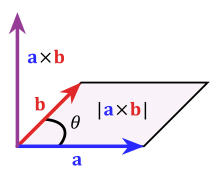
\includegraphics[width=0.30\textwidth]{crossproduct}
    \caption{The cross product}
\end{figure}

This seems a little strange. Why this definition of all things? It becomes a little clearer when we consider what the area of a parallelogram actually is.
This area is given by the base times the height, or for the vectors in the picture, $|\vec{A}| |\vec{B}|\sin(\theta)$, because $|\vec{A}|$ is the length of the base and $|\vec{B}|\sin(\theta)$ gives the height

So if the length of the cross product is this area, then $|\vec{A} \times \vec{B}| = |\vec{A}| |\vec{B}|\sin(\theta)$, and because we have introduced $\theta$, this becomes a very useful formula.

One use is to find the distance from a point and a line, which can be computed by crossing two vectors to form a parallelogram between the line and the point, and dividing by the length of its base to find the point's distance off the line.

It's worth specifically noting that the cross product returning an orthogonal vector is particularly powerful and useful. The length is arguably less useful of the two properties.

Actually computing this cross product is a little strange and unexplained to me, but I'll leave it here
\begin{align*}
    det
    \begin{vmatrix}
        \hat{i} & \hat{j} & \hat{k} \\
        A_1 & A_2 & A_3 \\
        B_1 & B_2 & B_3 \\
    \end{vmatrix}
\end{align*}

It's unclear to me why this produces an orthogonal vector, or why it is the length of the area of the parallelogram. Further research needed.

\subsection{Vector/Parametric Forms of Lines}

This is a short one. In $\mathbf{R}^2$, lines can be defined in point slope form. You start at a point, follow a slope, and you get your line. 
There's a similar concept in $\mathbf{R}^3$, with the vector form of a line. You start at a point, follow a vector, and you get your line.

The vector form of a line is as follows:
\begin{displaymath}
    L = \{\vec{r}(t) = P_0 + t\vec{d}\}
\end{displaymath}hatr of the line, the 3-space analog of a line's slope, and $t$ is some real number to scale the direction vector by.

This can also be rewritten in terms of each component of the vector that is returned by $\vec{r}(t)$, known as the parametric form of the line

\begin{gather*}
    x = P_{0x} + \vec{d}_xt\\
    y = P_{0y} + \vec{d}_yt\\
    z = P_{0z} + \vec{d}_zt\\
\end{gather*}


To compare to the other forms, all of the following draw the same line
\begin{gather*}
    y = x \\
    y - 0 = 1 (x - 0)\\
    L = \{\vec{r}(t) = (0, 0) + (1, 1)t\}\\
    \vec{r}(t)= (x, y): 
    \begin{cases}
        x = 0 + 1t\\
        y = 0 + 1t\\
    \end{cases}
\end{gather*}

As a sidenote, if you want to represent a line segement, instead of an infinite line, the idea is pretty cool. The line segement between two points starts at the first point and follows a vector formed by subtracting the points, and clamping $t$ between 0 and 1.

So the segment between $(a, b)$ and $(c, d)$ is represented by

\begin{gather*}
    \{\vec{r}(t) = (a,b) + t\left((c - a, d - b)\right)\}\\
    0 \leq t \leq 1
\end{gather*}

And checking this for $t = 1$ gives you 
\begin{displaymath}
    (a, b) + (c, d) - (a, b) = (c, d)
\end{displaymath}

And at 0 you get $(a, b)$, so the line will only exist between the two points. Pretty neat idea.

\subsection{Vector and 3D Functions}

Vector functions are pretty quick.
\begin{displaymath}
    \vec{v}(t) = (x(t), y(t), \dots)
\end{displaymath}

Their derivatives are the derivatives of the components of their vectors, and the usual derivative rules (product, quotient, etc.) work the way you would expect.

3D (or higher) functions are just as quick. Some function of x and y returns a z value, essentially taking the xy plane and raising it up along the z axis at each point $(x, y)$ to the value $f(x, y)$

If you want to take a derivative of these, you have to take some care, because there are now two axes in which you can move, so the notion of a derivative becomes a bit fuzzy. Enter the partial derivative

\textbf{Definition:} The partial derivative of a function is the derivative of a multidimensional function along a single axis. You take a slice of the surface created by the function, and the resulting single dimension of movement is the respect of the derivative. All other variables are treated as constants.

\begin{gather*}
    \frac{\partial}{\partial x}(f(x) = xy) = (1x^0)y \\
    \frac{\partial}{\partial y}(f(x) = xy) = x(1y^0)
\end{gather*}

\subsubsection{Tangent Planes and Linearization}
One of the uses of the derivative in 2 dimensions was to approximate a function. The tangent line is pretty close to the function at very small steps. In 3D, we need a tangent plane, to represent the two dimensions of movement we have.

To find a tangent line in $\textbf{R}^2$, we used a point and a slope $y - y_0 = f^\prime (x)(x-x_0)$. In $\textbf{R}^3$, we need two slopes, so 
\begin{displaymath}
    z - z_0 = \frac{\partial f}{\partial x}(x_0, y_0)(x - x_0) + \frac{\partial f}{\partial y}(x_0, y_0)(y - y_0)
\end{displaymath}
represents the tangent plane.

A little manipulation of that later and we get a way to linearize the function, which is pretty similar
\begin{displaymath}
    f(x, y) \approx f(a, b) + \frac{\partial f}{\partial x}(a, b)(x - a) + \frac{\partial f}{\partial y}(a, b)(y - b)
\end{displaymath}

Where $(a, b)$ is the point where you start, and $(x, y)$ is where you end up. Which amounts to starting at $(a, b)$, and walking a bit in the x multiplied by $\frac{\partial f}{\partial x}$, which is the slope (rise / run) in the x times the run, so you get the z that you should go up by, and you do the same in the y axis

We can think of tangent planes, tangent lines, and linearizations as applications of \textbf{differentials}. \textbf{Differentials} are generally linearizations of functions in whatever dimension the function is in. In two dimensions, the differential of a function is $dy = f^\prime (x)dx$, for any arbitrary dx. This gives you an equation for a tangent line. It's a slope times a change in the "run", so you get a rise.

In 3-space, the differential becomes slightly less clear because $f^\prime (x)$ now has to become partial derivatives. In 3-space $z$ changes instead of 2-space's $y$, but z can change in both the x and y axes. So to incorporate both of these, the total $dz$ will be dependent on $dz_x$ and $dz_y$.

We call then call $dz$ the total differential, defined by
\begin{gather*}
    dz = \frac{\partial f}{\partial x}(x, y)dx + \frac{\partial f}{\partial y}(x, y)dy  
\end{gather*}

This works out pretty well. When you bump x, what is the change in z. When you bump y, what is the change in z. The function that represents the total change in z is dependent on how much you bump x and y by. This then defines a tangent plane. You can bump x and y by any value, including zero, so this necessairly has to be a plane because it has to exist when either bump is zero, so it cannot be a line because it must be able to move independently in two axes. It also doesn't make sense to be a line. How are you going to represent two dimensions of potential change in a one dimensional object.

\subsubsection{Quadratic Approximation}
While we're doing linear approximations, we may as well touch on quadratic approximation.

Quadratic approximation approximates a 3D function as a paraboloid instead of a line. This is pretty useful, as it's a good idea to approximate a 3D function with a 3D figure, instead of 1D lines.

This approximation is just an extension of a taylor polynomial. It looks like:
\begin{displaymath}
    Q_f(x) = f(x_0) + \nabla f(x_0)\cdot(x-x_0)+\frac{1}{2}(x-x_0)^T\mathbf{H}_f(x_0)(x-x_0)
\end{displaymath}
That looks pretty scary, let's break it down.

First off, $f(x_0)$ is the value of the function at the point $x_0$. This is the y-intercept, so to speak, of the approximation, or the point at which we want to start the paraboloid.

To that, we add $\nabla f(x_0)\cdot(x-x_0)$. This is a linear term. It's a vector of partial derivatives dotted with a vector of changes in position from the point $x_0$. This will build a tangent plane. We add the change in z with a nudge in x, and the change in z with a nudge in y, together, to get the total z change at any point away from $x_0$, which will be rendered as a plane.

Finally, we add the scary quadratic term. The first thing we should break down is $\mathbf{H}_f(x_0)(x-x_0)$. $\mathbf{H}_f$ is the Hessian matrix of $f$, a symmetric and square matrix of second order partial derivatives.
We evalute $\mathbf{H}_f(x_0)$ to be those partial derivatives at $x_0$. We then multiply this matrix by a column vector of the same changes we had earlier. In 3D this works out as follows:
\begin{gather*}
    \mathbf{H}_f(x_0) = \begin{bmatrix}
        \frac{\partial f}{\partial xx} & \frac{\partial f}{\partial xy}\\
        \frac{\partial f}{\partial yx} & \frac{\partial f}{\partial yy}\\
    \end{bmatrix}\\
    \mathbf{H}_f(x_0) \cdot (x - x_0) = \begin{bmatrix}
        \frac{\partial f}{\partial xx}(x_0) \cdot (x - x_0) + \frac{\partial f}{\partial xy}(x_0) \cdot (y-y_0)\\
        \frac{\partial f}{\partial yx}(x_0) \cdot (x - x_0) + \frac{\partial f}{\partial yy}(x_0) \cdot (y-y_0)\\ 
    \end{bmatrix}\\
    \frac{1}{2}(x-x_0)^T\mathbf{H}_f(x_0) \cdot (x - x_0) = 
    [x-x_0, y-y_0] \cdot \begin{bmatrix}
        \frac{\partial f}{\partial xx}(x_0) \cdot (x - x_0) + \frac{\partial f}{\partial xy}(x_0) \cdot (y-y_0)\\
        \frac{\partial f}{\partial yx}(x_0) \cdot (x - x_0) + \frac{\partial f}{\partial yy}(x_0) \cdot (y-y_0)\\ 
    \end{bmatrix}\\
    = \frac{1}{2}\frac{\partial f}{\partial xx}(x_0) \cdot (x-x_0)^2 + \frac{1}{2}\frac{\partial f}{\partial yy}(x_0) \cdot (y-y_0)^2 + \frac{\partial f}{\partial xy}(x_0) \cdot (x-x_0)(y-y_0)
\end{gather*}

So what's this look like then? We have taylor polynomials along x and y, which makes sense. The third term is (kind of) a taylor polynomial along some combination of the x and y directions.

This is sufficient for any direction between the axes. If you consider how this is being computed, it's whatever change in x, and whatever change in y, times the "slope" when you move along a partial derivative. They aren't independent, though, they're multiplied. If they were independent this would be another linear term. Because they are multiplied, this will create a parabolic term. (Consider when the x change is identical to the y change to see this, you end up squaring the change)

This is all super shallow though, and I need to spend more time on it. Further research needed.
\subsubsection{Contour Maps}
\label{sssec:Contour Maps}
Before we leave 3D functions it's worth mentioning contour maps because they're cool.\\
\begin{figure}[h]
    \centering 
    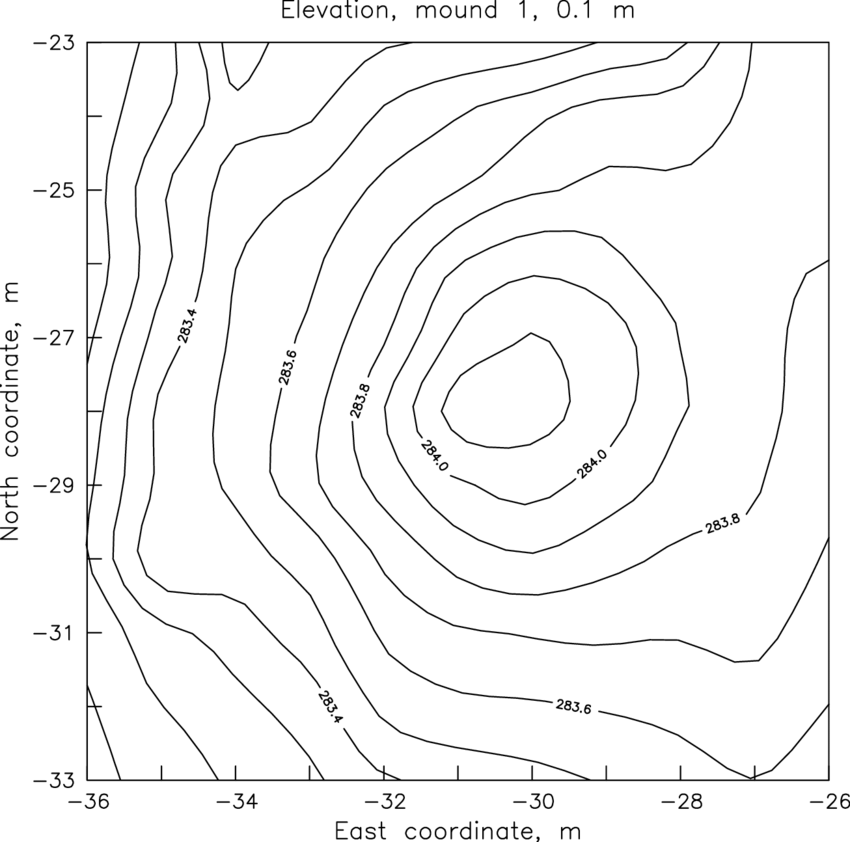
\includegraphics[width=0.5\textwidth]{contourmap}
    \caption{A contour map of some mound}
\end{figure}\\
The contour map of a 3D function is created by taking horizontal slices of the function at constant z values. This creates a neat way of visualizing these functions and will be useful for gradient fields later.

\newpage

\section{The Multidimensional Chain Rule}
What came before was all pretty clear the first time through. After this, though, was when the lectures started to get muddy, which inspired me to take some more detailed notes.

The multidimension chain rule is a weird one. I couldn't ever find a satisfactory answer, intuition, or explanation for why it made sense.

It helped to first consider the single dimension chain rule.

\begin{gather*}
    \text{For a function} f(g(x)), \text{Let } u = g(x) \\
    \frac{d}{dx} f(g(x)) = \frac{d}{dx} f(u) = f^\prime (u)\frac{du}{dx}\\
    \frac{du}{dx} = g^\prime (x)\\
    \frac{d}{dx} f(g(x)) = f^\prime (g(x)) g^\prime (x)
\end{gather*}

This is still pretty shallow for me. Seems more like a trick of notation than something that makes sense. If we go back and consider the derivative, though, it is definitionally the change in the value of the function when you change the input by a little bit.
\begin{gather*}
    f(x) = x^2\\
    f(x + dx) = (x+dx)^2\\
    = x^2 + 2xdx + {dx}^2\\
\end{gather*}

So when we nudge the input of the function by $dx$, we get $x^2 + 2xdx + {dx}^2$ as the height of the function at $x + dx$. Before the nudge, the function was $x^2$, so the nudge changes the function by adding $2xdx + dx^2$. As $dx \to 0$, the value of $dx^2$ becomes very small and much less significant than $2xdx$. So when we nudge the function, its return value meaningfully changes by twice the value of the function at x, times the tiny nudge we made in the x, meaning that $f^\prime (x) = 2x\ dx$. This is where the power rule comes from.

When we nudge $f(g(x))$, we first nudge $g(x)$ by something, and the new value then becomes the input of $f$.

Let's ignore $g(x)$ for a second. So long as $g(x)$ is differentiable, then a small change in x would feel no different than if we nudged $g(x)$, as far as $f$ is concerned. 
Let's call $g(x)$ $u$ instead. A small nudge in $u$, du, corresponds to a change of $f^\prime (u)\ du$. The nudge du is itself the change in $g$ when you change x, that nudge is $g^\prime (x)\ dx$, which gives us the chain rule

\begin{gather*}
    \frac{d}{dx} f(g(x)) = f^\prime (u)\ du\\
    du = \frac{du}{dx}dx = g^\prime (x) dx\\
    \frac{d}{dx} f(g(x)) = f^\prime (g(x)) g^\prime (x)\ dx
\end{gather*}

Okay, so with the single dimensional chain rule out of the way we still have a beast left. Let's look at something easy first.
\begin{gather*}
    \text{Let} f(a, b) = a + b\\
    \text{What is } \frac{\partial}{\partial x}f(x^2, y^3).
\end{gather*}

The first thing to note is that a and b are private variables. The user who is feeding x's and y's into f has only indirect control over a and b. This means that taking a partial derivative with respect to a or b means nothing here, because the user inputting variables only knows what x and y are, and has never heard of a and b

Now, if you're just looking at this, you can just plug the functions in.

\begin{gather*}
    f(x^2, y^3) = x^2 + y^3\\
    \frac{\partial f}{\partial x} = 2x \\
    \frac{\partial f}{\partial y} = 3y^2
\end{gather*}

So you dont actually \emph{need} the chain rule. You could plug all of the functions in and take a partial derivative as normal.
However, if your functions get complex, say $f(u, v) = u^2sin^2(v)$ and $u$ and $v$ are themselves complicated, the partial derivatives get annoying really fast, so having a way to pre-compute this with a formula would be nice.

Let's take that example. For $f(sin(x), cos(y))$ what happens when we nudge x? Let's again call sin(x) u.

\begin{gather*}
    f(u, \cos(y)) = u^2\sin^2(\cos(y))\\
    \frac{\partial f}{\partial u} = 2u(\sin^2(\cos(y))\ du\\
    du = \frac{du}{dx}dx = \cos(x) dx\\
    \frac{\partial f}{\partial u} = 2\sin(x)(\sin^2(\cos(y))\cos(x)\\
\end{gather*}

Okay, that's all fine and good I guess, but what does it actually mean? The first thing we did was ignore sin(x). We want a change in f with a change in x, but a change in x makes a change in u, so we considered the change in u first.
The change caused by u was $\frac{\partial f}{\partial u}$, which is some term times du. So what is du? We really want a change with respect to x, so how can we find du in terms of dx?
We can take $\frac{du}{dx}$, because u depends on the variable x, and then multiply that by dx, so that we're left with du.

So if $\frac{\partial f}{\partial u}$ is something times du, and du is $\frac{du}{dx} dx$, then $\frac{\partial f}{\partial x} = \frac{\partial f}{\partial u} \frac{du}{dx}$
This makes some sense. If we nudge x and it doubles u, and if we nudge u and it doubles f, it makes sense that nudging x quadruples f (by multiplying, not squaring/exponentiating).

This is nice, but what if v also depends on x? Then we also have to think about v now! So when we nudge x it makes some change to u, which makes a change to f, but it also makes a change to v, which makes a change to f. What's the total change?
Well u and v aren't really related. The function can do whatever it wants with u and v, but no matter what, when you take a partial derivative of one, the other is constant. Unless they're the same thing, but that's beside the point.
Because they create two independent changes, you just add them. You change x, it changes u, which changes f. It also changes v, which changes f. u and v don't change each other, so you don't multiply them or compose them or do anything fancy. The partial derivative is just the sum of the changes.

This is all honestly shallow intuition. I still don't really get all of this. My saving grace is this tree
\begin{figure}[h]
    \centering 
    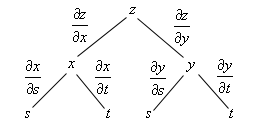
\includegraphics[width=0.5\textwidth]{chainruletree}
    \caption{How to compute a multidimensional chain rule}
\end{figure}

If you want \large$\frac{\partial z}{\partial s}$ \normalsize you follow all of the branches to s, multiply down the branch, and add the various branches. So,
\begin{gather*}
    \frac{\partial z}{\partial s} = \frac{\partial z}{\partial x} \frac{\partial x}{\partial s} + \frac{\partial z}{\partial y} \frac{\partial y}{\partial s}
\end{gather*}
This gives you what we had earlier. You keep unpacking various partial derivatives until you reach the variable you want, and then add all of the independent changes. I particularly like this tree becuase you could go 9 functions deep and it works the same way

My professor really likes emphasizing this derivative matrix $Df(x)$, which I think is supposed to be the \externalLink{https://en.wikipedia.org/wiki/Total_derivative}{Total Derivative} but everything about this seems like we'll get to it later so I'll skip it for now and instead focus on

\section{The Gradient and Directional Derivatives}
So first off, the gradient is, according to Grant Sanderson, weird. We'll start with the algebraic definition.

\begin{gather*}
    \nabla f(x, y, ...) = (\frac{\partial f}{\partial x}, \frac{\partial f}{\partial y}, \dots)
\end{gather*}

\begin{gather*}
    \text{Let} f(x, y) = x^2 sin(y)\\
    \frac{\partial f}{\partial x} = 2x\sin(y) \\
    \frac{\partial f}{\partial y} = x^2\cos(y) \\
    \nabla f(x, y) = (\frac{\partial f}{\partial x}, \frac{\partial f}{\partial y}) \\
    = (2x\sin(y), x^2\cos(y))
\end{gather*}

With this, it's important to note that the gradient is a \textbf{vector valued function}, which is a vector of all the partial derivatives of f. (Grant called this a full derivative, as it contains all of the partial derivatives).

A helpful way to think of this is
\begin{gather*}
    % \LARGE
    \nabla = \begin{bmatrix}
        \frac{\partial}{\partial x}\\
        \frac{\partial}{\partial y}\\
        \vdots
    \end{bmatrix}
    % \normalsize
\end{gather*}

And that $\nabla f(x)$ distributes $f(x)$ over that vector.

This is fine. It's a vector of partial derivatives, so what? What's neat about this is that it gives the direction of steepest ascent. That isn't at all intuitive at all, though. We just have a whole bunch of slopes in a whole bunch of directions. What gives?

First, a quick detour:

\subsection{Directional Derivatives}
What if instead of nudging a 3D function by x or y, we nudge it along some vector?
Pick some vector $\vec{v} = (a, b)$ to nudge along. This is like nudging by a in the x direction, and b in the y direction.
The directional derivative is
\begin{gather*}
    {\nabla}_{\vec{v}} f(x, y) 
    = a\frac{\partial f}{\partial x} + b\frac{\partial f}{\partial y} 
    = \vec{v} \cdot \nabla f(x, y)
\end{gather*}

Note the subscript of $\nabla$. Without it it's the gradient, as on the right, and with it it's the directional derivative.
Similar to a partial derivative, this corresponds to a slice of the graph of a 3D function from some plane that isn't necessarily parallel to either axis x or y.
That slice gives us some 2D function, where some step along that vector corresponds to a change in z, and some people write the directional vector as \Large $\frac{\partial f}{\partial \vec{v}}$ \normalsize to denote this.

That said, the line to remember is that the directional derivative is a partial derivative along some vector, instead of an axis. This is also results in giving you the slope of a graph when you walk along some vector, but you should be careful that when you are looking for the slope, you take a unit vector as the direction, otherwise you could get some multiple of the actual slope. 

Okay, with that in mind let's think about...

\subsection{Why the Gradient Gives the Direction of Steepest Ascent}

Imagine you are at a point on a 3D graph. In order to climb the graph as fast as possible, you want to find the largest slope from a directional derivative along some unit vector evaluated at your point. (A unit vector because $\vec{\infty}$ would always be the best choice)

To find this best vector, consider what the directional derivative actually is.

\begin{displaymath}
    \nabla_{\vec{v}} f(a, b) = \nabla f(a, b) \cdot \vec{v}
\end{displaymath}

If we want to maximize $\nabla_{\vec{v}} f(a, b)$, we really need to figure out what $\vec{v}$ dotted with $\nabla f(a, b)$ will give us the biggest slope (remember that $\vec{v}$ is a unit vector).

A dot product equals $|a| |b| \cos(\theta)$. When the vectors lie on the same line, ($\cos(\theta) = 1$) we get a maximal dot product, assuming $|a|\ \&\ |b|$ are fixed, which they are in a directional derivative.

Therefore, the best unit $\vec{v}$ will be on the same line as $\nabla f(a, b)$. It needs to be a unit vector, so take $\frac{\nabla f(a, b)}{|\nabla f(a, b)|}$ and you get a unit vector that returns the highest possible slope from a directional derivative

The gradient itself, evaluated at $(a, b)$, normalized, will then be the vector that, when traveled along, results in the greatest increase in altitude, because it is the highest slope, as we got from maximizing the directional derivative. Some more intuition is in the section on vector fields.

Pretty cool stuff. It's the backbone of the Gradient Descent Algorithm and I implemented it for a \externalLink{https://github.com/SAXTEN2011/LinearRegression/blob/master/index.js}{Linear Regression Model}

\subsection{Vector Fields}
\label{ssec:vectorFields}

Vector fields are pretty much what they sound like. It's a 2D plane of vectors, i.e. a function $f(x, y)$ that maps each point to some $\vec{v}$, which generalizes to some n-dimensional function mapping to some n-tuple

The construction of one such vector field can be done using the gradient operator. Taking $\nabla f(x, y)$ gives you some vector at the point $(x, y)$, and if you find the vector at every $(x, y)$ you get a vector field that we call the gradient field, because it was generated by the gradient operator. 

A neat thing to note is that the gradient field points in the direction of steepest ascent, because it is formed by the gradient. This is necessarily orthogonal to contour lines, as the steepest ascent is also the shortest path from one contour line to the next. If you zoom in super close on two nearby contour lines, they will eventually look like parallel lines. The shortest distance between parallel lines is an orthogonal path, so a gradient field will produce vectors orthogonal to a function's contour map.

\begin{figure}[h]
    \centering 
    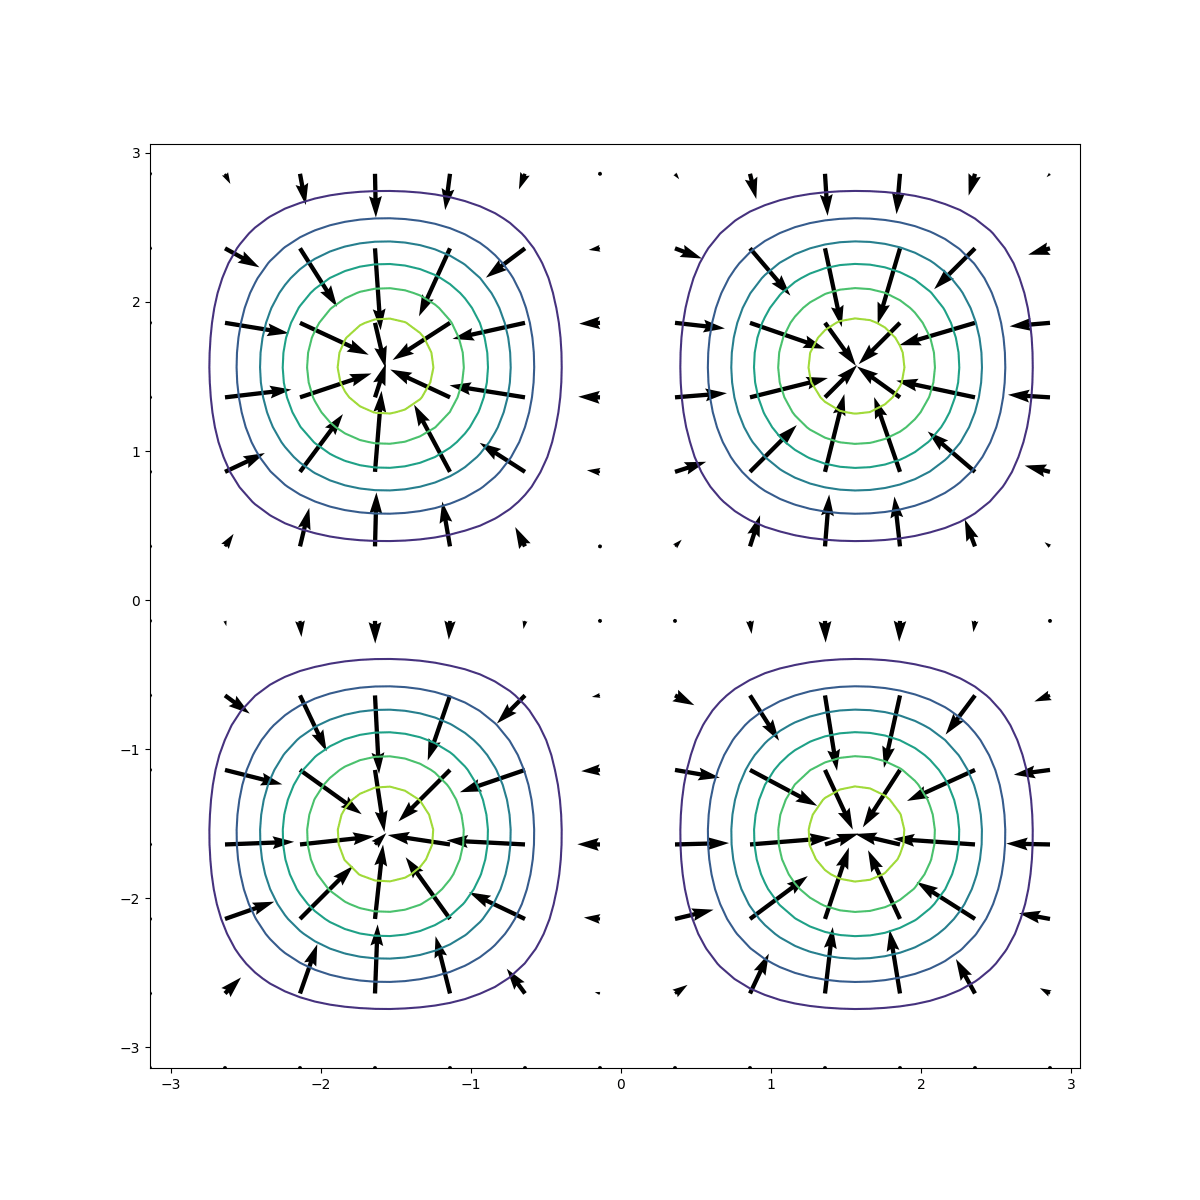
\includegraphics[width=0.75\textwidth]{orthogonalContour-min}
    \caption{A gradient field of $z = \sin(x)\sin(y)$ against its contour field. The vectors all point towards the peaks, which means orthogonal to the contours! Also, if they were parallel to the contours, you find a way to not ascend at all!}
\end{figure}

Okay so what. I get that being able to visualize a gradient field helps give some intuition for what following a gradient would mean, but why would I ever really need this outside of that intuition? 
The answer is on \externalLink{https://en.wikipedia.org/wiki/Vector_field\#Operations_on_vector_fields}{this wikipedia page} and I hope I take some notes on this. 
Further research needed.


\subsection{Tangent Planes to Level Surfaces}
If we want to find a tangent plane to a 3D surface, say $x^2 + y^2 + z^2 = 3$, we need to find some normal vector to the surface that we can make a plane from. To find this normal vector, we will be a little sneaky. We can think of this 3D function a level surface of a 4D function. A level surface is a slice in one axis of a function, so a level surface of a function, say $z = x^2 + y^2$, is just where $x^2 + y^2$ equals some constant $c$, i.e everywhere on the function that has a $z$ value equal to $c$, also known as a \hyperref[sssec:Contour Maps]{contour} of the function.

So we know that the gradient of a function points orthogonal to a contour line, because that is the fastest direction to the next contour line. Remember that the contour of a 3D function is some 2D curve, so the contour of a 4D curve is some 3D surface, and the gradient of a 4D function will result in a vector that is orthogonal to the 3D contour of the function. 

We can exploit this by thinking of some 3D surface as actually being some contour of a 4D function. So maybe we have some function $w = x^2 + y^2 + z^2$, in the 4D space defined by the axes x, y, z, and w. If we set $w$ to $3$, i.e take a level surface at $w=3$, then we get the sphere we led this section off with.

So to find a tangent plane to $x^2 + y^2 + z^2 = 3$, we should consider $x^2 + y^2 + z^2 = w$, a function of one higher dimension, and take a gradient. This will give a 3 vector that is necessarily orthogonal to the sphere because a 4D gradient will be orthogonal to its 3D contour. We can then use this gradient vector as the equation of a tangent plane $\vec{n}(p - p_0) = 0$, to find a tangent plane.

\section{Optimization}

In optimizing a function, we look for maximum and minimum values of the function. This is extremely useful across a wide range of use cases, the most prominent of which is probably machine learning.

\subsection{Finding Local Extrema}
In 2 dimensions this process is rather simple. You first find everywhere that the derivative is zero or undefined, so as to find points on the function where there is no direction you can move in to make your position better (whether better means a higher or lower altitude is up to you). You then check the second derivative of the function to see if the function is concave up (corresponding to a minima) or concave down (corresponding to a maxima).

In more than 2 dimensions we have the same general process. First we find where all partial derivatives are zero ($\nabla F(x, y) = \vec{0}$). If any of these partial derivatives weren't zero, then there would be a direction you could nudge the function in to increase or decrease the value of the function, thus your point is not an extrema. 
Put another way, the gradient points in the direction of steepest ascent, so if the gradient at a point is zero there is no direction that ascends, so you are at an extrema.
(Putting it this way sounds like it would only work at maxima. You can also get to minima by walking in the opposite direction to maxima, because the opposite direction of steepest ascent will be the steepest descent) 
It was surprising to me that the gradient being zero was sufficient. It seemed reasonable that your derivative in the X and Y could be zero but between those axes it wouldn't be. This is wrong though. If you take a directional derivative you dot the direction vector with the gradient. So if the gradient is zero, so are all of the directional derivatives. 

Once we find all of the critical points, we need to decide if these points are maxima, minima, or saddle points. To find this, we need a second derivative test.

To find the second derivative of a multidimensional function, let's find the derivative of the gradient. Each term will need to be derived with respect to every other element, so the gradient becomes a matrix,
\begin{align*}
    \nabla f &= \begin{bmatrix}
        \frac{\partial f}{\partial x}\\
        \frac{\partial f}{\partial y}
    \end{bmatrix}
    \xrightarrow{Becomes}
    \mathbf{H}_f = \begin{bmatrix}
        \frac{\partial f}{\partial xx} & \frac{\partial f}{\partial xy}\\
        \frac{\partial f}{\partial yx} & \frac{\partial f}{\partial yy}\\  
    \end{bmatrix}
\end{align*}

This matrix is called a Hessian Matrix, a symmetric matrix of the second order partial derivatives of a function. 
This is the equivalent of a second derivative of a multivariable function, and we can use it for a sense of concavity.
This will be very useful shortly.

If a critical point in 3D is a max or a min, the max/min will look like a paraboloid. If we find a taylor approximation of the 3D surface at a critical point, and the approximation looks like a paraboloid, then we know if it is indeed a max or a min, and its sign (whether the approximation is always positive or always negative) will distinguish between them.

We aren't really intersted in an accurate taylor approximation, we just want to try to fit a paraboloid to the surface and hope that it works. If it does work we've definitely got a max/min, and if it doesn't we almost certainly don't. Here's how we find this limited taylor approximation.

Firstly, we can linearly approximate the function. At any given point, the derivative with respect to some axis times the change in that axis will give a tangent line. In 3D we want a tangent plane instead of a line, so we dot the gradient with a vector formed by $(x, y, z) - p_0$, where $p_0$ is the point at which you are taking the derivative and $(x, y, z)$ represents some new position along each axis.

This spits out a plane, which tells us where the function is increasing and decreasing. At a critical point this must zero, because critical points necessarily have horizontal tangent planes, no increase or decrease as you nudge your coordinates.
We are doing this approximation specifically at critical points, so we can entirely ignore the linear part because of this.

So we look next at the concavity of the function, encoded by the second derivative. When you bump x, it changes the function's rate of change in the x proportional to it's second derivative.
If you take the new rate of change that the bump results in, and multiply that new rate of change by that bump again, you get the change in z caused by the second derivative.
It helps to think of this in units. If you are given acceleration, you need to multiply it by the time once to get a velocity, and again to get a position.
Meters per seconds squared, times seconds times seconds, gives you meters. In the same way, a second derivatives times a dx times a dx gives you a dz!

To represent this in 3D, we hit the hessian matrix on both sides with the change vector (in 2D we just multiply $f^{\prime \prime}$ by $(x - x_0)^2$). We've done lots of talking; here are some nice conscise symbols.

\begin{gather*}
    \text{Let } a = (x_0, y_0)\\
    f(x, y) \approx f(p_0) + \nabla f(p_0)(a - p_0) + \frac{1}{2}(a - p_0) \cdot \mathbf{H_f}(p_0)(a - p_0)
\end{gather*}
(the $\frac{1}{2}$ ensures that the derivative of the approximation is not twice the derivative of the actual function. 
This doesn't really matter in our case right now because it doesn't change the sign.)

But we only want to take this approximation at critical points, so $\nabla f$ is zero, and the linear term goes away!

So now our approximation is simply $f(p_0) + \frac{1}{2}(a - p_0) \cdot \mathbf{H_f}(p_0)(a - p_0)$

$f(p_0)$ is the height of the function at our critical point. If the second term is always positive, then we only add height when we move away from the point, so the critical point is a min, and if its a max then the second term must always be negative.

So now we can determine whether the function is a max/min by just looking at the sign of $(a - p_0) \cdot \mathbf{H_f}(p_0)(a - p_0)$, which is very nice!

So how do we find this sign? First let's figure out what that actually evaluates to.

After some multiplication that is both too long and too straightforward to write out, here is what we're left with in the 2 variable case
\begin{gather*}
    \frac{1}{2}f_{xx}(x_0, y_0)(x - x_0)^2 + f_{xy}(x_0, y_0)(x - x_0)(y - y_0) + \frac{1}{2}f_{yy}(x_0, y_0)(y - y_0)^2
\end{gather*}

That's pretty long. Because this is a quadratic form (i.e the product of two sums, for example $(a+b)^2$), let's write it as such.

\begin{gather*}
    ax^2 + 2bxy + cy^2
\end{gather*}
Where $a = \frac{1}{2}f_{xx}(x_0, y_0)$, $x = (x - x_0)$ and everything else follows in the same way.
(I think this is the first time I've used the $f_{xx}$ notation in these notes. This is equivalent to $\frac{\partial f}{\partial xx}$).

Note that we want to know where the \textit{evaluation} of the quadratic form is positive, not the slope or anything like that. 
We want to know this because we add the result of this to the height at our critical point. 
If the value of the approximation is always of the same sign, we can discern maxes and mins.

If a parabola (or paraboloid, but it's easier to consider 2D right now) is always positive, or always negative, it never crosses the x axis. A root of a function is definitionally when it crosses the x axis, so if this parabola has no solutions (or roots) then we know it is always the same sign and is definitely a min or a max.

But we're trying to approximate a 3D function, so we need to consider paraboloids for approximation, not parabolas. Thankfully, if a paraboloid crosses the x axis, then the slice of the paraboloid where y is some constant value where that crossing happens, then the resulting parabola from the slice will also have a root at the same place.

So to figure out if a paraboloid has a root, let's fix $y$ to be some $y_0$, so our quadratic form is now
\begin{gather*}
    ax^2 + 2bxy_0 + c(y_0)^2
\end{gather*}
So now we have a parabola (because it's only a function of a single variable, x, now), parameterized by some $y_0$. If we can't find a $y_0$ that gives this quadratic form roots, then we must have a max or a min, because no roots means not crossing the x axis which means the parabola is only positive or only negative.

Alright, let's find these roots then. Enter the old quadratic equation.

\begin{gather*}
    \frac{-2by_0 \pm \sqrt{(2by_0)^2 - 4ac(y_0^2)}}{2a} \\
    =\frac{-2by_0 \pm \sqrt{y_0^2 (4b^2 - 4ac)}}{2a}\\
    =y_0\left(\frac{-2b \pm 2\sqrt{b^2 - ac}}{2a}\right)\\
    =y_0\left(\frac{-b \pm \sqrt{b^2 - ac}}{a}\right)\\
\end{gather*}

This equation returns x values of solutions. If this value is not real, there aren't any solutions. This formula will never be real if $b^2 - ac$ is negative, because the square root of a negative is imaginary.

The obvious problem here is when $y_0$ is zero. This is problematic because it smooths over other solutions. If there was also a root at, say, $x=1$, it would get multiplied by zero, so the test will be inconclusive.

If the test is conclusive (i.e. $y_0$ isn't 0), we return back to needing to know when $b^2 - ac < 0$, in order to find when our paraboloid has no real solutions. We're pretty abstracted now, so let's fill back in a, b, and c with their actual values.
\begin{gather*}
    b^2 - ac = (\frac{1}{2}f_{xy})^2 - (\frac{1}{2}f_{xx} \cdot \frac{1}{2}f_{yy})\\
    = \frac{1}{4}f_{xy}^2 - \frac{1}{4}f_{xx}f_{yy}\\
\end{gather*}

So now we want to find when $\frac{1}{4}f_{xy}^2 - \frac{1}{4}f_{xx}f_{yy} < 0$. This is equivalent to
\begin{gather*}
    f_{xy}^2 - f_{xx}f_{yy} < 0 \\
    f_{xx}f_{yy} - f_{xy}^2 > 0
\end{gather*}
We make these changes because it puts the statement exactly in the form of the determinant of the Hessian matrix! That's pretty crazy. The determinant of the hessian will determine if a quadratic approximation at a critical point does or does not have solutions. If the approximation has no solutions, then the paraboloid is always positvely or negatively valued, and thus is a max or a min.

We can finally determine whether this is actually a max or a min by looking at either of $f_{xx}$ or $f_{yy}$. We know with absolute certainty that this point is either a max or a min,
and as a result know that the approximation at this critical point is a paraboloid. A paraboloid can't have one concavity in one axis and a different concavity in another,
so looking at either second order partial derivative will tell us directly if the paraboloid is concave up, or concave down, and we can then make the final call whether a critical point is a max or a min.

Okay, okay, that was super long. Let's recap.
We have a function and want to know where the local maxes and mins are.
These will happen at critical points ($\nabla f = \vec{0}$), but we need to figure out if each critical point is a max or a min.
To find out if it's a max or a min, we will try to approximate the function with a paraboloid.
If that paraboloid is always positively valued we have a min, and oppositely for a max.
That paraboloid can't always be positively valued if it crosses the xy plane.
We can find where that paraboloid crosses the xy plane by finding the solutions to the paraboloid.
We can find these solutions from the quadratic formula, and because the quadratic formula takes a square root of $f_{xy}^2 - f_{xx}f_{yy}$, we can force the paraboloid to not have solutions if that value is negative.
That value just so happens to be the \textbf{negative} determinant of the hessian matrix, so the opposite sign of the determinant of the hessian matrix is also the sign of the bit under the square root of the quadratic equation.
If the determinant is positive, then the bit under the square root is negative.
Negative square roots aren't real, so the paraboloid has no solutions, therefore never crosses the xy plane, therefore is always positively valued (or always be negatively valued), and we must really have a min (or a max)!

The textbook will not write all of that out, and will just give the following rule:
\begin{enumerate}
    \item If the determinant of the hessian is positive, then the sign of $f_{xx}$ tells you whether it's a max or a min.
    \item If the determinant is negative, then we have a saddle point (because there's a crit point but it isn't a max or a min)
    \item If the determinant is zero, the paraboloid might have solutions, who knows, so the test is inconclusive.
\end{enumerate}
To elaborate on point 1 a bit, if the determinant of the hessian is positive, the paraboloid has no solutions. 
If the paraboloid has no solutions, then it never switches sign. 
Because it never switches sign no matter what, all points near the paraboloid have the same concavity.
If they didn't, the approximation wouldn't have worked out to have no solutions.
We fit this paraboloid based on the partial derivatives, so we knew from the start it would follow their concavity, but we didn't know if everything else between them agreed, or even if they agreed themselves.
When the paraboloid has no solutions, every direction from the critical point has the same concavity, so we can just pick any one of those directions to figure out if we're at a min or a max.
For some reason conventions says to pick xx, but you could just as easily pick yy.
No matter which direction you pick, a positive value means a min, and a negative value means a max.
\subsection{Finding Absolute Extrema}
When we look at critical points and second derivatives we are finding local extrema, places on the function where there are no bumps to your input you can make to gain or lose altitude.

If we want to look for the highest point anywhere on the curve, the absolute maximum (or minimum), we need to do some thinking first.
For example, what's the absolute maximum of $f(x) = sin(x)$? Well there are a lot of them. Infinitely many of them, actually.
What if we wanted to know the absolute maximum and absolute minimum values of $f(x) = \frac{1}{x}$? This is even less clear.
Is infinity a value? Is that the absolute max and negative infinity is the absolute min? If so, at what x value do those extrema happen at?
It's not zero, but any value that's not zero can always get a little closer to zero, and increase the altitude of the function, and therefore can't be an extrema.

It would really help if we just said that we want to find the absolute extrema on some closed interval.
When we consider the absolute extrema in some interval, there are two places we can find these extrema.
First, the critical points will give us local maxes and mins. 
These maxes and mins may well have the biggest or smallest height of the function at their points, but we aren't guaranteed this.
If you chop the function off at the end of some interval, you could chop it off at some really big value that would have kept getting bigger outside of the interval
(For example, chopping $x^2$ at any value outside of zero will put absolute maxes at the endpoints of the interval). 
But these chopped points won't be critical points, because they weren't local extrema, just large values that would have been larger outside of the bound.
We need to specifically look for these points when searching for absolute maximum/minimum values because they won't show up when we solve for critical points.

So to find the absolute extrema of a function, we take all of the critical points, and all of the endpoints of our closed interval, and find the biggest and smallest values among them.
We actually don't even need to check whether the critical points are actually local maxes or mins. We can just find all of their values and take the biggest and smallest.
We might as well just evalute the function at the critical points instead of dealing with second derivative tests.
We are, after all, looking for the biggest and smallest heights of the function.
Who cares if that happens at a saddle point or not.

In 2D evaluating a function at the endpoints of an interval is super easy. If the interval is $[0, 1]$, then you just take $f(0)$ and $f(1)$.
In 3D, life isn't as easy\footnote{Is it ever?}.
We need to slice the surface along some direction or curve or whatever defines our interval.
So maybe the interval we care about is the unit circle (points with distance 1 from the origin), or a square from $(0, 0)$ to $(1, 1)$.
In each of these cases, we need to take some kind of slice of the function, which will give us a 2D function and then find the absolute extrema on that 2D function!
So there you have to find the critical points of the 2D slice, evaluate it at its endpoints, and it's a real pain.
This all sounds like I'm leading up to some nice trick. I'm not. I hope there's a better solution out there though.
Further research needed.

So the overall process for finding 3D absolute extrema goes as follows:
\begin{enumerate}
    \item Find the critical points
    \item Find any suspicious points on the boundary of the interval
    \item Evaluate the function at all of the points you collected from the first two steps. The biggest and smallest values are your absolute extrema.
\end{enumerate}
The suspicious points are places on the boundary of the interval that might be extreme values.
The boundaries are 2D slices of the function, so you should just find the absolute max/min on that 2D slice, and throw that in the pot with the critical points of the surface inside the interval.
Finding absolute extrema then becomes a nested problem.
You need to consider all of the extreme values within the 3D surface bounded by the interval \emph{and} all of the extreme values on the 2D boundary slices. 

\subsection{Constrained Optimization}
This is the form of optimization that makes up all the fun word problems.
You're always either building a box with maximal volume and a fixed amount of cardboard,
or the biggest pen for your cows with a fixed amount of fence.

Whatever the random problem the professor came up with is, you need to find the optimal inputs given some constraint.
The textbooks, in an effort to make you work as hard as possible, call the function you want to optimize f, and the constraint function g.
This was frustratingly abstract to me. The idea is pretty obvious, but is obscured by notation.

What was strangest to me was the notion of a constraint function.
The easiest example of a constraint function is representing how much cardboard you have to build a box.
If L, W, and H, are the length, width, and height of the box, then your constraint function might look like
\begin{gather*}
    g(L, W, H) = 2LW + 4WH
\end{gather*}
Which represents twice the cardboard to make the base, and 4 times the cardboard to make a wall.
In other words, the amount of cardboard it takes to build you box.
So why can't you just say that you only have 12 square feet of cardboard and not bother with this function?
It's actually a useful construction.

If you take a level surface of $g$ at 12, that represents having only 12 square feet of cardboard.
If you plug in your L, W, and H, to $g$, it tells you if you are within the constraint.
If you use 5000 square feet of cardboard, that doesn't equal 12, and your constrait function will be a contradiction. 
Put another way, if you find some optimal point on $f$, and that point isn't on the level curve of $g$, then you can't use that point.
This lets us reduce our problem to finding the absolute maximum value on $f$, constrained to points on $g$.

But this isn't so clear. We take a level surface at $g = 12$ (12 is just some random value that I'm taking for an example),
this level surface is 2D. That can't really intersect with $f$, which is a 3D surface.
It can, however, intersect with contour lines of $f$.
We could also just say that we care where the x and y values of points on f are also points on g,
or even say that we extend the level surface of g to be a cylinder so that we can find meaningful intersections,
but thinking about it as a contour map is a really useful perspective. 

When a level surface of $g$ (which I am going to just call $g$ from here on out) crosses a contour line of f we can figure out a couple of things.
First, we know that the point at which they intersect is a candidate for the optimal point.
This is because the point at which they intersect is necessarily on f and g, and we are trying to find the optimal point that satisfies exactly this fact.
However, we can also immediately disqualify this point!
If $g$ \emph{crosses} a contour line of $f$ it must be moving to another contour line somewhere else.
This value \emph{has} to be bigger or smaller than the point at which the lines crossed, because if the new value wasn't different than the value at which we crossed the contour line, then it would have to be on the contour line.
But it isn't on the contour line because we crossed the contour line, so we're moving to bigger and better places if we follow $g$, so we keep following $g$.
When do we stop then? If $g$ just barely touches a contour of $f$, i.e $g$ is tangent to a contour of $f$, then $g$ is always less than (or greater than) the value of that contour line, except when $g$ touches that value, in which case it is a local optima!
That's huge news! When $g$ is tangent to a contour of $f$, we find a local optima. So let's just find all of those local optima, evaluate the function at all of the points, and pick out the best value.

We can find these by considering what it means for two curves to be tangent to each other. 
The tangent line of the curves must be parallel, and the curves must share a point.
If they don't share a point, they can't be tangent, and if their tangent lines at the point that they share aren't parallel, then you could follow the tangent line to get inside of the other curve.
The curves being tangent means that you cannot do that. 
Put another way, the tangent line is a linear approximation. 
If the linear approximation of both functions are parallel, the functions don't cross over into each other. 
I am having a difficult time justifying this fact and \textbf{need to rewrite it}.

So where are tangent lines to contour maps parallel? 
Well first off, how do we even get tangent lines to contour maps?
The gradient will spit these out, as we talked about earlier on in the notes.
So now we just need to find where the gradient vectors of $f$ and $g$ (the function, not the level surface at 12), are parallel.
Vectors are parallel if one is a multiple of another, so we can express this as
\begin{gather*}
    \nabla f(x, y) = \lambda \nabla g(x, y)
\end{gather*}
Where solutions are the critical points of the function.
This might not be enough information.
Frequently we can solve for lambda, but not x or y.
In order to solve for x or y, we can also go back to our constraint function, and consider the system
\begin{displaymath}
    \begin{cases}
        \nabla f(x, y) = \lambda \nabla g(x, y) \\
        g(x, y) = 12
    \end{cases} 
\end{displaymath}
It's important that this system also has the constraint function in it, because it constrains solutions to only those that satisfy g.
If you only looked at $\nabla f(x, y) = \lambda \nabla g(x, y)$, you could find solutions well outside the constraint.
Because $g$ equals some constant, we can find x or y in terms of lambda, plug the lambda value into $g$, and solve for the other variable, which will be a definite value.
Then we have cocnrete values for x and y, evaluate the function at that point, and find the maximum and minimum values between those to find our absolute extreme values.

\subsection{Constrained Optimization With Two Constraints}
The process is almost exactly the same, except that it takes the following form:
\begin{gather*}
    \nabla f(x, y) = \lambda \nabla g(x, y) + \mu \nabla h(x, y)
\end{gather*}
Where $g$ and $h$ are constraint functions. My big question was "why addition?"

Wikipedia's article says to consider the constraint functions to be two lines.
The intersection of those lines will be the only point that satisfies both constraints, and will thus be the max.
However, these lines can't share a tangent line to each other (they wouldn't intersect), so it can't be possible that contours f, g, and h, all share a tangent line, which is what I initially thought multiple constraint solving would look like.
In this case, the gradient of f needs to be some linear combination of the gradient of the other two constraints, and multiple constraints generalize in the same way.

Further research needed as to why this makes sense.

\section{Multiple Integrals}
In 2D we can find areas under curves with integrals, and that's super useful!
For example, It's used all over the place in \externalLink{https://github.com/SAXTEN2011/GyroLib2020}{GyroLib} to find theta from angular velocity.
It's always handy to be able to climb up the position/velocity/acceleration tower, in the same way that it's useful to go down it with derivatives.

In 3D we look for volumes under surfaces, instead of areas under 2D curves.

From 2D, we added a whole bunch of rectangles of height $f(x)$ and width $dx$. 
In 3D, we use rectangular prisms of height $f(x, y)$, length $dx$ and width $dy$.

Another nice way to do this is to add up areas under slices of the surface. 
We can fix some y value to $y_0$ and take the corresponding slice of the function.
Integrating this 2D function gives us the area of that slice.
If we now consider $y_0$ to be the variable $y$, we can integrate that integral over y.
This adds up the areas of all of the slices of the functions, and gives us a volume.

Given that adding up slices in the x or slices in the y measures the same volume, the order of integrating doesn't really matter, except when it does.
Fubini's Theorem dictates when it matters, but it's not super relevant right now.
Everything we're given to compute in class will work just fine both ways.

To actually compute multiple integrals, you perform something called...
\subsection{Iterated Integrals}
Iterated Integrals are how we actually find the volume under a surface.
Let's look at an example
\begin{gather*}
    \int_c^d \int_a^b f(x, y) \,dx\,dy
\end{gather*}
To compute this, you take $\int_a^b f(x, y) \,dx$ and compute it. We'll call the result $u$.
You then compute $\int_c^d u\,dy$ to find the final volume.

Here's an example with numbers!
\begin{gather*}
    \int_0^1 \int_0^1 (x+y) \,dy\,dx\\
    = \int_0^1 xy + \frac{1}{2}y^2 \biggr \rvert_0^1 \,dx\\
    = \int_0^1 x + \frac{1}{2}\ \,dx\\
    = \frac{1}{2}x^2 + \frac{1}{2}x \biggr \rvert_0^1\\
    = \frac{1}{2} + \frac{1}{2} = 1
\end{gather*}

\subsection{Integrating Over a General Region}
Sometimes we want to integrate over nicely shaped domains like rectangles, as we did above.
This is pretty straightforward.
Sometimes we want to integrate over crazy squiggly lake shaped things.
This is not so straightforward.

When we integrate over some region (say between two sine waves, i.e $sin(x)$ and $sin(x) + 5$ we might actually have to be mindful of our integrals.
If we take vertical (y direction) slices of our domain, we're fine.
Horizontal (x direction) slices, however, could intersect the sine wave, and all of the sudden our integral is way off.

In these cases, we need to consider the shape of the function to make sure we are taking slices of the function that make sense.
This is like performing the vertical line test.
If we pass a horizontal (or vertical) line across the domain, and intersect the domain in a nontrivial way, we can't take slices in that direction.

Visualizing the domain is the easiest way to determine which direction you should take slices in. 
It's not that hard to see which axis will give you trouble. 
The more tricky part is knowing if your problem axis goes first or second.
Remember that the outside integral is what adds up slices, so if you're going along the y axis to add slices (i.e your outside integral is w.r.t y), then you must be adding up slices that are parallel to the x axis.
Similarly, if you are adding up slices as you move along the x axis, you must be slicing in the y direction.
So your slice direction is the inside integral, so that the outside integral moves orthogonal to that direction to compute a volume.
\textbf{Problem axes become outside integrals.}

For example, the problem axis in figure 6 is the x axis.
\begin{figure}[h]
    \centering 
    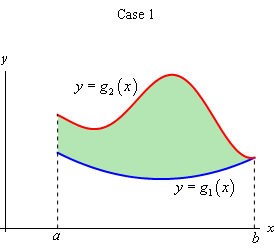
\includegraphics[width=0.5\textwidth]{problemaxis}
    \caption{}
\end{figure}
It might be easier to think of it as the problem direction, instead of an axis, but whichever way you think about it, you want to take vertical slices.

How do you take a vertical slice? 
You integrate with respect to y!
That tripped me up a lot. If you integrate with respect to x in 2D you get slices parallel to the y axis.
So what gives? Why does integrating w.r.t y in 3D produce vertical slices of the function all of the sudden?
When you integrate w.r.t y in 3D, you hold x to be a constant. This gives you a 2D function in the yz plane.
The base of that graph is the y axis, so you end up slicing the domain of integration along the y axis as well.
That slice is represented as:
\begin{gather*}
    \int_{g_1(x)}^{g_2(x)} f(x, y) \,dy
\end{gather*}
You then apply your outside integral over x to add up all of those y slices.
\begin{gather*}
    \int_a^b\left(\int_{g_1(x)}^{g_2(x)} f(x, y) \,dy\right)\,dx
\end{gather*}

A final way to see this is that the domain is between two functions of x. 
If you try to integrate that with respect to x, the bounds \emph{and the function} depend on x, and that is potentially impossible?
Just avoid all of that by integrating w.r.t y first.

Hold on. What if I want to integrate over a square whose edges are sine waves?
Every axis is a problem axis!

If at all possible, try not to want to do this. However, here is how you would do this.

Just like in 2D, you can add integrals together to get areas,
so the integral from 0 to 1, plus the integral from 1 to 2, is the same as the integral from 0 to 2, assuming no funny business.
In 3D we have the same principle. If you integrate over two adjacent domains, and add their integrals, it's like integrating over both of them in one step.
So now just split your square into a whole bunch of domains that have only a single problem axis (maybe one domain between the top and bottom sine wave, one domain as the area of the left sine wave and a third as the area of the right sine wave).

You also could do some thinking about whether the sine waved sides change the area or not.
If they cover a full period it might be identical to a normal square with lines as sides.
Frequently, you can think about properties like that (symmetry is a common one as well) to cheat the integral a bit.

\subsection{Changing Order of Iterated Integrals}
For some reason, you might want to change the order of iterated integrals. 
Maybe the math is easier when you integrate x first, and then do y, or maybe it's easier the other way around.

If you're integrating over some strange bounds, pretty much anything but a rectangle, the process isn't so easy.
Say you want to integrate over some squiggly shaped domain.
You need to take slices of the function in a different direction, which will require new bounds to be computed.

\textbf{The following is conjecture}

If you are integrating over a domain, you are almost certainly integrating between two functions on the inside, and two numbers on the outside.
If you want to switch this around, the easiest way is, again, to visualize the domain.
For the same reasons as before, the inside integral will be a function, but now of the other variable.
This function is definitionally the inverse of the functions before.
If one function of x is above the other function of x, then as a function of y it must be lower.
To see this, rotate a graph by 90 degrees. The lower function comes out on top.
Because the functions switch around, you also need to switch your bounds around, so it seems that you take the inverse of the functions, and switch the order of the bounds.

Finally, you need to find the new outside bounds. 
The bounds used to be x values, but now they're y values.
To find these new values, we can use our old functions.
The bounds just need to be the endpoints of the function, so we can evaluate our old functions at their old bounds to find the bounds of the rotated function.

\subsection{A Few Application of Double Integrals}
\subsubsection{Area of 2D Domains}
If you find the volume of a cylinder of some sort, it is equal to the base of the cylinder times the height.

If you force the height of that cylinder to be 1, then the volume of the cylinder will equal the 2D area of the base.
To find the volume of some cylinder, you integrate some curve that defines the height of that cylinder over the 2D base.
If that function is $f(x, y) = 1$, then the height at all points is 1, and thus integrating that function over a domain will result in the area of the domain.

So the general formula is:
\begin{gather*}
    \text{Area} = \iint_{\mathbf{D}} 1\,dx\,dy
\end{gather*}

\subsubsection{Surface area}
If we want to find the surface area of some curve, we can think about shingling it like a roof.
If we tesselate a whole bunch of squares, and add up their areas, we can get a nice approximation of the surface area.
This just begs for an integral to be used, but how do we express these squares?

Let's think about some different curves. Firstly, a horizontal plane will have some surface area, let's call it $A$.
If we take that surface area and pull up a hill from it, the surface area has to increase.
If you hammer a bump into a sheet of metal, the sheet has to deform, because this hill has more surface area over it's domain than just a flat plane.
We can just add area in magic math land, so we say that some sheet with a bump in it has an area greater than $A$.

Thus, the higher the slope at each point, the bigger the shingle will be. 
If we didn't think about the slope at each point, we are just adding up constant area squares at each point, which will just give us the area if we projected the surface to the xy plane.

Instead, let's think about how we fit these shingles on the curve.
For every point, we need to build a shingle that connects a rectangle from the point you consider to some next dx and dy.
We can express these points as starting at $(a, b)$ and adding $(dx, 0, f_{x}(a, b)dx)$ and $(0, dy, f_{y}(a, b)dy)$.
In other words, we take a tangent plane, and just take a teeny tiny shingle out of that big plane.

But now we need the area of this square.
It is spanned by $(dx, 0, f_{x}(a, b)dx)$ and $(0, dy, f_{y}(a, b)dy)$, so the cross product will definitionally spit that out.

So our integral looks like 
\begin{gather*}
\iint \lVert(dx, 0, f_{x}(a, b)dx) \times (0, dy, f_{y}(a, b)dy)\rVert    
\end{gather*}
But that is one heck of a cross product to compute, so let's simplify it a bit.

The cross product comes out to 
\begin{gather*}
    (-f_x dxdy, -f_ydxdy, dxdy)
\end{gather*}
The length of that cross product is the area of the shingle
\begin{gather*}
    \sqrt{(dxdy)^2(f_x^2 + f_y^2 + 1)}\\
    = \sqrt{f_x^2 + f_y^2 + 1}\,dxdy
\end{gather*}
Remember that $f_{x}$ and $f_y$ are evaluated at each point $(a, b)$. 
Gets pretty busy to write their full function calls out for all of this.

This is also the distance from the origin of the point $(f_x, f_y, 1)$ in 3-space. 
I wonder if that is significant in some way. Further research needed.

\subsection{Integrals in Polar Coordinates}
If you need to integrate over circles, it's time to bust out the polar coordinates.
Circles in cartesian end up with weird exponents and radicals and stuff, and polar makes this way easier.

You can convert by substituting all x for $r\cos(\theta)$ and all y for $r\sin(\theta)$.
Usually you can just eyeball it by remembering that $r^2$ is $x^2 + y^2$.

Integrals are little weird now that we're in polar. 
It's kinda hard to get squares out of polar coordinates, so it's not clear how we actually take this integral.
In cartesian, it's easy to sum up the areas of rectangles times the height of the function, but we have circles now.
But circles look a lot like straight lines if you zoom in far enough.
If we bump r by some value, and theta by some other value, we will move in something like a diagonal.
That fact is hard to justify, so it's probably false, but it is just enough intuition for me to not question it much.

That diagonal will cover some square's diagonal, so what's the area of the square?

First off, we've bumped theta by some value. 
The corresponding change in the y will be $r\sin(d\theta)$ but we are bumping theta by some teeny value, so by the small angle theorem (one of my very favorite theorems),
we can say that the square(it's really a rectangle) has height $rd\theta$.

So what's the change in x?
Good question. We need to stop thinking of this square as being parallel to the x and y axes.
It's actually rotated along the radius, so at 45deg the square is also rotated 45deg.
This makes it pretty clear that the width of the squre will be $dr$, because the rectangle is defined along that axis.

Now that we've changed our perspective a bit, is our height still right?
It is, actually, because $d\theta$ will form a teeny tiny triangle that is also rotated to the value of big theta, so we're still good.

Quick recap of all of that, some teeny $d\theta$ will form a triangle because the arc of the circle that is created by $d\theta$ is basically just the tangent line as we get infinitely small.
That triangle has a height of $rsin(d\theta)$, because it's a triangle.
Extending off of that height is also some $dr$. Because that triangle's base is defined by r, the width of the square that we add after adding $dr$ and $d\theta$ will just be $dr$.

Here's a picture to show that, straight from the textbook.
\begin{figure}[h]
    \centering 
    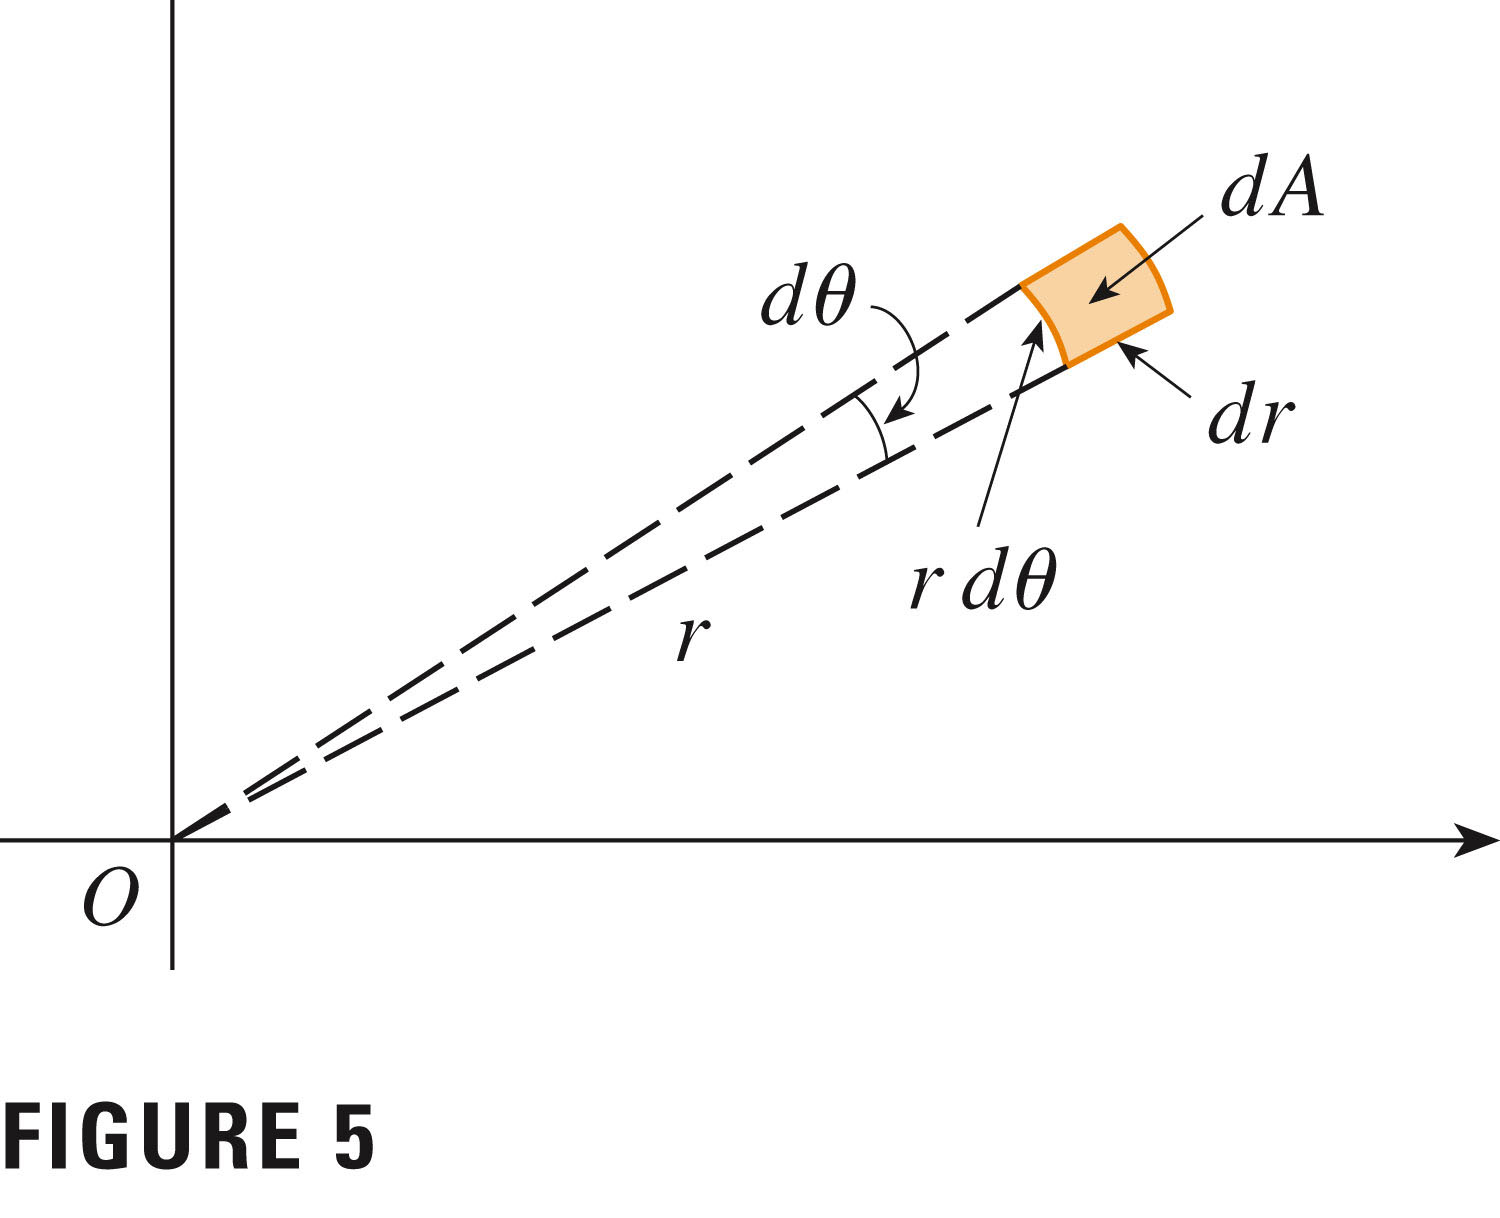
\includegraphics[width=0.5\textwidth]{polarIntegral}
    \caption{This is figure 5 from the textbook but its actually figure 7}
\end{figure}
The super important thing is to remember how to find the area of that little square.
The base is $dr$, and the height is $rd\theta$
So to add up volumes, you multiply the base ($rdrd\theta$), where $r$ is the radius at that point, and multiply it by the height of your function.

All said, it comes out to
\begin{gather*}
    \iint f(r, \theta)\,rdrd\theta
\end{gather*}

\subsection{Triple Integrals}
Triple integrals follow so easily from double integrals that it might be fair enough to put a triple integral on a test if you only learned double integrals, just to check your understanding

There is, however, one teeny complication.
If you need to integrate over some really crazy 3D volume, we get some problems.
\subsubsection{Triple Integrals Over General Regions}
Thankfully, we have a saving grace.
If you can figure out our lower and upper bound of z given x and y, you reduce the problem back to 2D again.
Usually, it's not that hard given the textbook problems, so the general strategy should be to
\begin{enumerate}
    \item Integrate first by z. Figure out the bounds of z as a function of x and y
    \item Project your domain to the xy plane and find the bounds like a double integral
\end{enumerate}
If you can pull that off, you can save yourself a lot of thinking
\subsection{Integrals in Cylindrical, Spherical coordinates, and the Jacobian}
When we take any integral in any coordinate system, we really just need to consider how to add up volumes in that space.
Namely, what is the volume of the box created by the nudges in any axis.

I wrote about how you do this in polar coordinates, where the significant part is that the box made by $dr$ and $d\theta$ has area $rdrd\theta$.
Let's look at two other coordinate systems (3D systems, instead of 2D) and figure out how to integrate over them.

\subsubsection{Cylindrical}
Cylindrical is a 3D extension of polar. 
In polar we take an r and a $\theta$ to find 2D points.
If we just assign each of those points some z value we get spherical coordinates.
So you can represent any point in 3-space as $(r, \theta, z)$,
and to convert from cartesian to cylindrical it looks exactly like cartesian to polar.
$x$ becomes $r\cos(\theta)$ and $y$ becomes $r\sin(\theta)$ and z stays as z.

How we integrate in cylindrical falls out pretty naturally, because it's just polar with a z value, the volume of the boxes is the base (which comes from a polar system),
and the height, which is just z.
So the area of cylindrical boxes is base times height, where base is $r dr d\theta$, from polar, and the height is $dz$, because it's cartesian.

All said, the triple integral to remember is...
\begin{displaymath}
    \iiint f(x) \,rdr\,d\theta\,dz
\end{displaymath}
In whatever order is necessary or convenient.

\subsubsection{Spherical}
Spherical is also an extension of polar, with a little more complexity.

We take a polar coordinate system, and raise each point to some theta against the z axis.
We represent these points as $(r, \theta, \phi)$.
We take some radius, rotate it along the xy plane, and rotate it along the z direction, to correctly set the x, y, and z values of a point.

Except that's not the whole truth, because rotating a point from the xy plane towards the z axis necessarily decreases the x and y values!
So where are those points actually at?
It's not as simple as $r\cos(\theta)$ and variants of that, because the z value (which is influenced by $\phi$) changes the x and y.
So with that observation we know that x and y must rely on both $\theta$ and $\phi$.

Thankfully, the relationship is pretty easy.
Imagine that $\phi = \frac{\pi}{2}$ (lies on the xy plane, no z value), then we just have polar coordinates living ambiently in 3D.
In this case, x and y \emph{do} equal r times their trig function, because z exercises no influence over them.

Now imagine that $\phi = 0$, then the point must lie on the z axis.
If it lies on the z axis, you can rotate the point along the xy plane all you want and nothing is going to happen,
so the polar portion of the spherical coordinates should be irrelevant.

If you are willing to squint your eyes a little, it just so happens that $\sin(\phi) = 1$ for $\phi = \frac{\pi}{2}$,
and $\sin(\phi) = 0$ for $\phi = 0$, so you could multiply $r\cos(\theta)$ and $r\sin(\theta)$ both by $\sin(\phi)$.
Then they are full valued when there's no z component, and gone when it's only a z component.

Another way you can think about this is that decreasing $\phi$ (rotating towards z axis from xy plane)
will decrease r, because r definitionally points away from the z axis, and you are moving it closer towards it.
That increase will be proportional to the sine of $\phi$, because $r\sin\phi$ is parallel to the xy plane.
The angle points upwards, after all.

With that out of the way, we can translate between cartesian and spherical as follows:
\begin{gather*}
    x = r\cos(\theta)\sin(\phi)\\
    y = r\sin(\theta)\sin(\phi)\\
    z = r\cos(\phi)
\end{gather*}

So if we want to integrate over a spherical domain, we need a way to compute the volume of a teeny tiny box of this sphere.
It's not so hard, though.
If we integrate in cartesian, the box has volume $dxdydz$, and we just wrote x, y, and z, in terms of spherical variables.
Let's just compute $dx$, $dy$, and $dz$, and multiply them!

However, each of x, y, and z has more than one variable.

- Quick shift in tone, I thought at this point that I was horribly off track, but
I took the gradient of x, y, and z, and took the triple product $z \cdot (x \times y)$ and it gave me $-r^2 \sin(\phi)$.
I think the negative was a calculation error somewhere, but that is exactly correct for the extra volume.
Assuming that this is actually a sign error, and not a fluke that happenened to get close by some wrong derivative, this feels pretty miraculous.
I'm a bit astonished that worked.

That was an absolutely nasty triple product to compute, though.
Only Wolfram could output that it reduced down nicely, so we need a better way of thinking about it, for re-derivation's sake.

We're about to talk about the Jacobian, which will generalize all of this, so I'm going to leave this one to dirty intuition.

We decided that in polar, boxes have volume $rdrdtheta$.
We also add some angle towards the z axis, $\phi$, so we need to add $d\phi$

After that, you need to figure out the change in z given a bump in $\phi$.
One way to justify this is that $d\phi$ is a quantity of radians, and radians don't help when we measure volume, we need units of volume, so we need to hit that radians number with a radius.
This means we add another $r$, in order to convert $d\phi$ from radians to our unit of volume.
Finally, when we increase $\phi$, we also scale everything else in the xy by $\sin(\phi)$ so we throw that in there too, to end up with
\begin{gather*}
    \iiint\, (rd\phi \sin(\phi)) rdrd\theta
\end{gather*} 
(All of the new stuff is in parenthesis).
Rearranging that to finish with
\begin{gather*}
    \iiint\, r^2 \sin(\phi) dr d\phi d\theta
\end{gather*}

\subsubsection{The Jacobian}
Here we go. 
The Jacobian will, for these purposes, generalize the process of finding those subdivisions of a volume that allowed us to integrate over things like spherical coordinates.

Quick intuition on matricies as transformations of space before we begin.
A matrix
\begin{gather*}
    \begin{pmatrix}
        2 & -3 & 1\\
        5 & 2 & 3\\
        1 & 1 & 1\\
    \end{pmatrix}
\end{gather*}

Represents a transformation of space, where sandard basis vectors $\hat{i}$, $\hat{j}$, $\hat{k}$,
map to the first, second, and third columns of that matrix, respectively.
This represents a change of basis, of sorts, that we get a new coordinate system with basis vectors
$(2, 5, 1)$, $(-3, 2, 1)$, and $(1, 1, 1)$.

This will form a basis because any vector can be written as a sum of basis vectors.
If we take any vector, and write it as a linear combination of the standard basis, we can perform the transformation over each basis vector in that sum and reach any vector
(much in the same way that we did in talking about \hyperref[equOfDotProductDefinitions]{the equivalence of the different definitions of the dot product}).

Great, with that out of the way, let's think about some crazy transformation that actually isn't linear at all.
Maybe it sends x to the sine of something and y to the sine of something else, and it's complete nonsense (maybe something circular).
So long as you don't have something truly insane, you can zoom in on some teeny tiny point (we seem to do that a lot)
and find what looks a whole lot like a linear transformation if you zoom in far enough that the curves become pretty much their tangent lines.

However, that linear transformation isn't going to be obvious. 
You could zoom in and the lines could be going in any random direction (but only one, because it's a linear transformation), so it's useful to figure out what that transformation actually looks like.

(To motivate doing this this, it will help us figure out how to find little chunks of crazy things, by converting something, say a polar coordinate grid, to a grid of squares that we can add up.)
The way we can do this is to linearize the function!
We were doing transformations before, so let's figure out a matrix that takes some tiny step in the standard basis, and tells you where that step would end up taking you after a crazy transformation.

Let's think about 2D.
If we are at some point in space before a transformation, and we move to the right by some nudge $dx$,
our overall change is $dx\hat{i}$, some scalar multiple of the basis vector.
We are thinking of linear transformations as mappings of basis vectors to other basis vectors, so this is very useful.

Recall what we're doing here - we have some crazy transformation, and we want to zooming way in on a tiny bit, in an effort to make it sufficiently linear.
So when we take a vector $dx\hat{i}$, we want to transform that vector to the change vector after the transformation.

We know exactly what this transformation is. 
Say we are sending $(1, 0)$ to $(a, b)$.
Where $a$ and $b$ are some function evaluated at $(1, 0)$.
If we take the partial derivatives of the function that spit out a and b with respect to x, we get the associated changes in the output vector given a change in x,
and the same works for y, so the Jacobian will be formed by taking the transformation and taking partial derivatives for each function that an input variable maps to.

These functions are commonly called $u$ and $v$, so we take
\begin{gather*}
    \begin{pmatrix}
        \frac{\partial u}{\partial x} & \frac{\partial u}{\partial y}\\
        \frac{\partial v}{\partial x} & \frac{\partial v}{\partial y}\\
    \end{pmatrix}
\end{gather*}

And when we take the determinant of this matrix, we get the factor by which it scales area.

So if we think of the transformation $(x, y) \mapsto (r\cos(\theta), r\sin(\theta))$ (cartesian to polar),
the Jacobian looks like
\begin{gather*}
    \begin{pmatrix}
        \frac{\partial}{\partial r} r\cos(\theta) & \frac{\partial}{\partial r} r\sin(\theta)\\
        \frac{\partial}{\partial \theta} r\cos(\theta) & \frac{\partial}{\partial \theta} r\sin(\theta)\\
    \end{pmatrix}
\end{gather*}

And if we take the determinant, we get $r\cos^2(\theta)dr d\theta + r\sin^2(\theta)drd\theta$, which is equivalent to
$rdrd\theta(\cos^2(\theta) + \sin^2(\theta))$, which is just $rdrd\theta$!

(We added the $dr$s and $d\theta$s as a figment of the chain rule, because they could mean something, or they could just be 1. 
Either way, it's useful to include in order to get all of what we want out of it)

So areas of little linear squares in polar have area $rdrd\theta$!
That's so cool! We found that earlier!
All we had to do was zoom way in until the coordinates looked sufficiently linear,
and represent that new linear looking coordinate system as a transformation from the standard basis to our zoomed in linear form.
After that, the area of each of the tiny squares could be found by taking the determinant, because the determinant is the factor by which area is scaled,
and we care about basis vectors, who will form squares of area 1, so the area of the subdivided squares is equal to 1 times the determinant, which is just the determinant.

\section{Vector Calculus}
So far the calculus we have been doing is just mostly generalizing calc 1 to more than two dimensions.

Vector calculus is our first departure from this, where we will operate on vectors and vector fields, instead of real numbers and coordinate planes.

We've already talked about vector fields in \textbf{\ref{ssec:vectorFields}}, but they will be immediately useful.
As a quick recap, a vector field is a space where points in the space are mapped to vectors.
$\nabla f(x, y)$ is an example of one such field, where every point maps to its gradient vector. 

\subsection{Divergence and Curl}
({I am heavily referencing \externalLink{https://www.youtube.com/watch?v=rB83DpBJQsE}{this 3b1b video} for this section. You may well watch it instead})


When you get to looking at vector fields you begin to quickly imagine following them in a path, or maybe more helpfully as some kind of flow.
Like if you dropped a ball, or a stream of water, on the field and it followed the vectors, you could kind of trace a path through the field.

If it rains on our field, and we get water poured everywhere, it's a neat question to ask where the water would end up pooling.

We can introduce the notion of divergence.
If a given point has a positive divergence, water is flowing out of that point, whereas if the divergence is negative (think of it as convergence, the opposite of divergence)
then water is flowing into that point, and it pools there.

But divergence isn't just about where the water stops.
While it's moving towards these pools, it moves at different rates.
Maybe it falls off of a waterfall, and moves slowly to get there, but falls very fast once the water is off of the fall.
We would say that waterfall has high divergence, because water leaves faster than it enters.

So the divergence is a number, a score that you give a point, that tells you how water is going to behave near that point.
It's positive if water goes away (diverges from the point) or negative if it comes in (converges into the point).
This is close to a derivative, where the little neighborhood around our point is what gives us the information about the divergence.

(As a quick sidenote, real water flow has a divergence of zero everywhere, because water fills up the point that it flows into.
If you put water into a full hole, an equal amount of water comes out.
Try not to think about that, though.)

For the curl at a point, we also think about fluid flow, but we want to know about how the fluid rotates around the point.
So if you drop a leaf onto the water, will it rotate clockwise, counterclockwise, or not at all?
Counterclockwise rotation is said to have positive curl, becuase it follows the unit circle, or its theta increases by a positive amount each second.
Clockwise rotation happens when you decrease theta, so it's called negative curl.
Don't mistake these for like vortexes or something, though.
If fluid flows faster at the top of a leaf than the bottom, it will rotate clockwise, so curl isn't just something for whirlpools.
If you drop a ping pong ball into the water, you also need to think about how the ping pong ball will spin in the other direction, too.
If water is flowing from front to back, it will rotate oppositely if water is flowing from back to front, so it's useful to represent curl as a vector,
where it points in the 3D direction of spin, because you can spin a ping-pong ball both horizontally and vertically.

With that intuition in the back of our heads, let's figure out how to actually compute them. We'll start with divergence.

\subsubsection{Computing Divergence}
For a point with positive divergence, water flowing into a point flows slower than water flowing out. 
So if we have water only flowing in the x direction, from left to right, our divergence is zero if the flow to the left has the same velocity as the flow to the right.
If the flow to the right is bigger than on the left, then we have positive divergence.
In other words, the value just to the left of the point is lower than the value just to the right.
If we were to graph that value, that would mean that going from left to right across the point increases the height of the graph, which exactly means that the derivative is positive.
And if flow is flowing from right to left (we'll call that negative flow) then positive divergence happens when left is more negative than the right.
Or put another way, going from left to right makes you less negative, therefore more positive, therefore again a positive derivative.

So from all of that we see that divergence will look at the derivative across a point.
In that example we only looked at water flowing in the x direction, so we would say that the partial derivative with respect to x at that point gives us our x divergence, the higher the partial derivative, the faster water flows out than in, and so the higher the divergence.

The same works for the y direction, that the partial derivative gives us the divergence in that axis as well.

When these derivatives agree, say they are both positive, then water will flow diagonally in the positive directions in both axes.
If they are equal and opposite, we want there to be no divergence, because water flowing from left to right may speed up, but water flowing bottom top slows down.
The net change on the water's velocity is zero, because the water is sped up in the x exactly as much as it's slowed down in the y.
Finally, if we have a highly positive divergence in the x, but a low and potentially negative divergence in the y, we want to consider the net change in the water across the point,
so adding the divergence allows us to consider that, too.

This leads us to want to add up the partial derivatives at the point, so we want to dot $\nabla$ with the value of the vector field at that point, in order to add up its partial derivatives.
In adding that up, we get a measure of the net change in velocity of water flowing across that point from any direction. 

So we can notate the computation of divergence as
\begin{gather*}
    \text{div}(x, y) = \nabla \cdot \vec{\mathbf{F}}(x, y)
\end{gather*}

If that didn't feel satisfying enough, it's almost exactly a transcription of \externalLink{https://www.khanacademy.org/math/multivariable-calculus/multivariable-derivatives/divergence-grant-videos/v/divergence-formula-part-2}{this video from grant},
which has some very pretty visuals and animations to go along with it.

\subsubsection{Computing Curl}
(Again, \externalLink{https://www.khanacademy.org/math/multivariable-calculus/multivariable-derivatives/curl-grant-videos/v/2d-curl-formula}{this KhanAcademy video is really great})

To compute curl, we are looking for places where the vectors around some point looks like they're going to spin.
When the vectors will create some spinning motion, the left vector has to point up, the top vector points left, the left vector points down, and the bottom vector points right.
All vector point into the next.

In order for all vectors to point to the next, the top and bottom vectors have to point oppositely,
and the left and right vectors also have to point oppositely.

But it doesn't have to be completely oppositely.
If water flows faster on the bottom than the top, you spin counterclockwise, so really we just care when the top goes faster than the bottom, and if the bottom just so happens to be negative, it still satisfies that.

We measure this in much the same way we measured divergence.
If we take a partial derivative across that point, and it increases, then we know we went from negative to positive (or low to high).

But the partial derivative we care about is a little goofy.
We want to know when the vector's x component (because the bottom vector needs to point to the right) increases as we go up.
If our vector field is $\vec{\mathbf{F}}(x, y) = (Q, P)$, and $Q$ and $P$ are some functions, then we care about $\frac{\partial Q}{\partial y}$. 

And similarly, $\frac{\partial P}{\partial x}$, will also tell us if the right vector has more vertical push than the left vector.

If the top pushes to the right, and the right pushes up, the water won't really spin.
You shove stuff into the corner.
So we need to know when $\frac{\partial Q}{\partial y}$ is opposite of $\frac{\partial P}{\partial x}$,
otherwise you end up shoved into the corner.

If they're opposite, then subtracting one from the other will tell you just how different they are from each other.
And if going from bottom to top increases the x component of the vector (think negative x at the bottom and positive on the top), you get clockwise rotation.
We call clockwise rotation negative, so we want to subtract that from the derivative across the horizontal direction, so that counterclockwise remains positive.

And that will just give us a number.
Kind of an angular velocity, how many radians you add per second.
If we think back to the initial intuition of curl, we also thought about putting a ping pong ball on the water.
If water is rushing under the bottom of that ball, the ball will spin into the water.
And just a single number doesn't describe the full extent of that rotation, because the ping pong ball can rotate horizontally and vertically,
and they can be independent, so one number can't possibly describe that rotation.

So we start to use vectors, as a way to get a 2D number to describe both possible axes of rotation.

This vector happens to be $\nabla \times \vec{\mathbf{F}}$, seemingly as a notational trick.
I have an extremely hard time imagining this really meaning anything other than a nice way to write the computation.

I really need to come back to this and think some more on it, but I need to think about anything else for a bit.
Even Grant kind of threw up his hands in the Khan Academy lecture, so I don't feel too bad about leaving it at just this.
If you aren't me and you're reading this, I have almost certainly forgotten to come back.

\subsection{The "real" definition of divergence and curl}
In defining how to actually compute divergence and curl, we played some notational tricks.
We started using vectors that didn't have numbers and determinants of matricies with vectors and numbers and partial differential operators as elements.
That breaks the rules a little, and it breaks them for good reason.
Thinking about curl and divergence as some product of $\nabla$ and $\vec{\mathbf{F}}$ is nice and easy to compute.
What follows is the more formal, less cheaty, way to define divergence and curl.

We'll start with (2D) divergence, whose formula is pretty nasty.
\begin{gather*}
    \text{div}\,\vec{\mathbf{F}}(x, y) = \lim_{\left| A_{(x, y)} \right| \to 0} \frac{1}{\left| A_{(x, y)} \right|} \oint_C \vec{\mathbf{F}} \cdot \hat{n}\, ds
\end{gather*}
So we start out pretty scary.
First off, let's define all of the random symbols.
$\vec{\mathbf{F}}$ is the vector field.

$(x, y)$ is some point on the plane

$A_{(x, y)}$ is a region of the xy plane, which includes $(x, y)$ somewhere inside it (hence the subscript)

$\left|A_{(x, y)}\right|$ is the area of the region

The limit term means we consider the limit as the area shrinks to zero, i.e. we shrink $A$ down to $(x, y)$

$C$ is the boundary of the region, the curve that defines the edge of it.

And the line integral $\oint_C \vec{\mathbf{F}} \cdot \hat{n}\, ds$ is the 2D flux of $\vec{\mathbf{F}}$ through the boundary of the region, called $C$

With all of that defined, it's time to figure out what it all means and does.
Again, this is the formula for divergence, the tendency for fluid to flow away from a point.

\textbf{I need to learn a whole bunch of stuff abount line integrals before I even think more about this.}


\subsection{Line Integrals}
\subsubsection{Over Scalar Spaces}
When we were doing normal integrals, say in 2D, we added up all of the subareas of the function on some interval.

In 3D, we added up all of the subvolumes that exist on some domain.

We could also consider that domain to be a curve, in which case the machinery we had for computing integrals over regions doesn't really help us, so we'll invent some machinery and call it a line integral.

When we integrate along a curve, we are trying to find the area of the curtain/fence/sheet of paper that is created by connecting the curve on the 2D plane
all the way up to the height of the surface above.

We just need to do a normal integral over this, but with some careful consideration about how to make the rectangles.

First off, we want a way to be able to turn this curve into a function of one variable, because the curtain/fence/sheet of paper is itself a 2D object,
and we take 2D integrals against one variable.
If we can find the parametric equation of the curve, then we can integrate with respect to t and all is well.

Finding this parametric equation isn't so bad either.
If you have a simple function like $y = x^2 + 5x + 2$, then you can parametrize this equation super easily by just letting $x = t$,
so that your parameterization is $x = t, y = t^2 + 5t + 2$, which will give you the same curve.
And it's important to remember exactly why we want this parameterization.
When we integrate, we add areas of rectangles at every point on the curve.
This parametric equation will allow us to easily hit all points just by scaling $t$.

Our integral, then, will look something like
\begin{gather*}
    \int_{t=a}^{t=b} \text{something} \, dt
\end{gather*}

So this integral will hit every point on our curve, but now we need to construct the rectangles.
Every $dt$ results in some nudge along the function.
$dt$ will nudge both the x and y values so as to keep along the function.
The nudge forms the base of our rectangle when we integrate, so we need to find the length of that nudge, and finding it is simple enough.
It's just the distance from our start point to the nudge, which looks like
\begin{gather*}
    \sqrt{\frac{\partial x}{\partial t}^2 + \frac{\partial y}{\partial t}^2}
\end{gather*}
Where $x$ and $y$ are the parametric equations of our curve $C$.

Now that we have the base, we just multiply it by the height, which is definitionally the height of the surface, so we finish with an integral that looks like
\begin{gather*}
    \int_{t=a}^{t=b} f(x, y, z) \sqrt{\frac{\partial x}{\partial t}^2 + \frac{\partial y}{\partial t}^2} \, dt
\end{gather*}
Which, to recap, finds the area of the curtain/fence/sheet of paper created from the curve on the xy plane that is stretched up to reach the 3D surface.
That area is computed by adding up rectangles of height $f(x, y, z)$, from the surface, and base formed by the length of a nudge in t, and a nudge in t nudges both x and y, because they both depend on t.
So that base becomes the distance from our start point, to a new point on the curve after some nudge $dt$

\subsubsection{Over Vector Fields}
When we integrate over curves in space, we are interested in finding areas and volumes, and that's all very nice and straightforward.
We can also integrate over vector fields (every single explanation of line integrals over vector fields loves to point out that 
it's used for computing work done by a force, but I don't really know what work is, so that isn't helpful).

When we take line integrals over vector fields, we draw a path throuh the vector field (because that's what a line integral cares about)
and along that path measure just how helpful the vector field is being at each point.
We can measure this by knowing where we are going (the derivative will tell us that) and then asking how much the vector from the field at this point is helping us get there.
If the vector is pointing in the opposite direction it's negatively helpful, and if it's pointing exactly where we are about to be, it's maximally helpful.

One way to interpret this is to think about sailing across the ocean.
If we dictate a path, the line integral gives us a score of how easy it will be to take this path.
If the score is high, then the ocean is helping us along by pushing us in the direction of our desired path.
If the ocean is still, we have to do all of the work ourselves, so it's a neutral score,
and if the ocean is actively pushing us perpendicular off of our path the whole time, we have to work extra hard to stay on the path, so it's negatively easy.

It's not too hard to sum this one up.
Like a normal line integral, if we can just parameterize the curve, the integral is as easy as
\begin{gather*}
    \int_{t=a}^{t=b} \vec{\mathbf{F}}(r(t)) \cdot \vec{r}^{\,\prime} (t) \, dt
\end{gather*}
Where $\vec{r}(t)$ is the parameterized function,
which means that $\vec{r}^{\,\prime} (t)$ is the tangent vector at that point, which tells us where we end up next.
When we dot the value of the vector field with the tangent vector to the curve at the point that we're standing on, we get a metric of how helpful the field is being.

And again, this returns a scalar which represents that helpfulness score, which makes sense because we are adding up a whole bunch of dot products.

\subsubsection{The Fundamental Theorem of Line Integrals}
I don't like how people teach the fundamental theorems of calculus.
I'll try a very slightly different take.

If you take the gradient of a function $f$, this gives you a vector field that points in the direction of steepest ascent.

If you walk along that vector field in any path (let's imagine the surface is above you, and the arrows are on flat ground), you can know how much you're climbing just by looking at the vectors on the ground.
If you walk exactly along the vector, you add that vector to your height.
If you walk opposite that vector, you can subtract it.
And anywhere in between lets you know what portion of the steepest ascent you are walking.

The key insight here is that vectors in a gradient field represent changes in height.
Traveling along vectors changes your height by that vector.

When you travel along any path on that gradient field, you know how much you would be climbing the function by if you just look at those vectors.
So one way to find the height difference between two points on a surface is to walk a path between those points on the gradient field,
and becuase the vectors in that field point towards the best direction to ascend, you can take a component of each gradient vector that you touch to know how much you ascend,
even if you don't follow that vector exactly.

When you take a path between two points, and walk along it adding up the component of the ascent vectors that you are following, it becomes clear that the path doesn't actually matter.
The difference in heights between two points is completely independent on how you walk from the first point to the second.
If you go down a valley before climbing up to your point, the changes will cancel out.
Because you are measuring \emph{all} of your changes in height as you walk, downs will cancel ups.

If we just write out that idea in notation, we are taking a line integral over any path between points $P$ and $Q$.
And along that path we add up the component of the gradient vector that we walk along.
\begin{gather*}
    \int_{t=a}^{t=b} \nabla f(r(t)) \cdot \vec{r}^{\,\prime} (t) \, dt
\end{gather*}
And that integral equals the difference in height, so we know that 
\begin{gather*}
    \int_{t=a}^{t=b} \nabla f(r(t)) \cdot \vec{r}^{\,\prime} (t) \, dt = f(Q) - F(P)
\end{gather*}
if $P$ and $Q$ are your start and endpoints, i.e. $P = \vec{r}(a)$ and $Q = \vec{r}(b)$.

Just remember that this only works if the field is conservative.
A conservative vector field is created when the field is the gradient field of some function, so a conservative vector field represents changes in heights.
If your field represents heights, the path doesn't matter.

\subsection{Green's Theorem}
Green's theorem is extremely cool and really easy to understand if you have just enough intuition.
I LOVE stuff like this.

Imagine some weirdly shaped domain over a vector field.
Green's theorem states that the line integral around the edge of that domain is the same as adding up the curl of every point in that domain.

Here's why that makes sense.

First off, the line integral around the edge of the domain tells you how helpful the vector field is along the path carved out by the edge of that domain.
So if you are a boat sailing over the ocean represented by the vector field, and the path your boat takes is the edge of the domain, the line integral tells you how much the ocean helps you along that path.

The other part of Green's theorem is that said line integral is the same as adding up the curl of every point in that domain.
What gives? Why's that the case?

Let's first imagine the path itself having curl.
A path with curl might mean that if you just sit on the path, like the baggage claim at an airport, it will pull you around the path, and the speed at which we do that is called the curl of the path.

Green's theorem says that adding up every point's curl in the domain will calculate the curl of the path on the edge of the domain.

First off, if the path is just a point, then of course the point has the same curl as the path.

If there are two points, side by side, let's think about what the sum of their curl looks like.

Imagine both points have positive curl, and the points are side by side, touching each other.
Point 1 is on the left, point 2 is on the right.
Because they have positive curl, the vectors that neighbor the points point in a circle, such that the vector to the left of the point points down, and to the right points up.
\begin{figure}[!h]
    \centering
    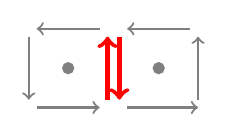
\begin{tikzpicture}
        \draw[gray, thick, ->] (0, 0.9) -- (0, 0.1);
        \draw[gray, thick, ->] (0.9, 1) -- (0.1, 1);
        \draw[red, ultra thick, ->] (1, 0.1) -- (1, 0.9);
        \draw[gray, thick, ->] (0.1, 0) -- (0.9, 0);
        \filldraw [gray] (0.5, 0.5) circle (2pt);
    
    
        \draw[red, ultra thick, ->] (1.15, 0.9) -- (1.15, 0.1);
        \draw[gray, thick, ->] (2.05, 1) -- (1.25, 1);
        \draw[gray, thick, ->] (2.15, 0.1) -- (2.15, 0.9);
        \draw[gray, thick, ->] (1.25, 0) -- (2.15, 0);
        \filldraw [gray] (1.65, 0.5) circle (2pt);
    \end{tikzpicture}
\end{figure}

See the red vectors?
They point oppositely.
So adding up those curls will cancel those vectors, so for a path around those two points only the perimeter will be considered.
This is exactly what we want, and it extends further.
You could imagine two more squares like that being tiled down and all of the interval vectors will cancel.
As these squares get infinitely small, we can tile them into the domain, so that addding all of them up will give us the curl of a path of the edge of a domain.

So how do we compute this?
How do we actually go about adding all of these curls?
Why, we need to add up infinitely small segements of a domain, so why not do a double integral!

So for a vector field that maps $(x, y) \mapsto (P(x, y), Q(x, y))$, we know from earlier that the curl is given by
\begin{gather*}
    \frac{\partial Q}{\partial x} - \frac{\partial P}{\partial y}
\end{gather*}

So to add all of those curls up, we just take a basic double integral
\begin{gather*}
    \iint_D \frac{\partial Q}{\partial x} - \frac{\partial P}{\partial y}\, dA
\end{gather*}
Pretty sweet. I love this one.
To write the full thing out
\begin{gather*}
    \oint_C \vec{\textbf{F}} \cdot \vec{ds} = \oint_C P\,dx + Q\,dy = \iint_D \frac{\partial Q}{\partial x} - \frac{\partial P}{\partial y}\, dA
\end{gather*}

Knowing this intuition also makes it pretty clear what happens when you have holes in your domain.
Like if you have a circlular domain with a circle cut out of its center, you just subtract off the integral of the region that isn't in the domain.
It's important you do that because the border of the cut out hole is getting canceled when it shouldn't, so you need to un-cancel it by subtracting its curl.
\end{document}